\documentclass[00_nsf_proposal.tex]{subfiles}
\hypersetup{
    colorlinks=true,
    linkcolor=blue,
    filecolor=magenta,      
    urlcolor=blue,
    pdftitle={Overleaf Example},
    pdfpagemode=FullScreen,
    }
\usepackage{tikz, booktabs, threeparttable}
\usepackage{hyperref}
\usetikzlibrary{calc}
\usepackage{natbib}
\usepackage{eso-pic}

\definecolor{maroon}{RGB}{128, 0, 0}
% Define the footer command with the red bar and logo.
\newcommand{\eraufooter}{%
  \AddToShipoutPictureBG{%
    \begin{tikzpicture}[remember picture,overlay]
      % Draw a red rectangle at the bottom of the page (2cm high)
      \fill[maroon] (current page.south west) rectangle ([yshift=2cm]current page.south east);
      % Place the logo centered within the red bar by shifting 1cm upward (vertical center)
      \node at ($(current page.south west)!0.5!(current page.south east)+(0,1cm)$) {%
        \includegraphics[width=0.25\linewidth]{figs/uc-logo-white.eps}%
      };
    \end{tikzpicture}%
  }%
}

% Activate the footer on every page.
\eraufooter

\begin{document}

\resetSectionPageNumber{Project Summary}
\section{Balance-Sheet Capacity and Cross-Strategy Treasury Arbitrage: SLR Exclusion Event Study
}

\subsubsection{Author}
Bailey Meche, Department of Economics, Masters in Computational Social Science - Economics, \href{mailto:baileymeche@uchicago.edu}{baileymeche@uchicago.edu}

\subsection{Abstract}
Regulatory leverage constraints are often described as shaping financial intermediaries’ willingness
and ability to intermediate U.S. Treasury markets, especially during stress episodes. The empirical
focus of this study is the Federal Reserve's
temporary exclusion of U.S.\ Treasury securities and Federal Reserve deposits
from the Supplementary Leverage Ratio (SLR) denominator---effective April~1,
2020 and expiring March~31, 2021---as a time-dated, plausibly exogenous shock
to balance-sheet capacity for covered bank holding companies. Using a pooled
difference-in-differences design across 17 daily arbitrage spread series in
four strategy classes (Treasury spot-futures, TIPS-Treasury, covered interest
parity, and equity spot-futures), I test whether the SLR relief differentially
compressed Treasury-based arbitrage spreads relative to non-Treasury controls.

The expiry of the exclusion is the paper's cleanest identification of price impact on arbitrage spread series. When the relief expired, Treasury-based spreads widened by $3.84$ basis points more
than non-Treasury spreads in the subsequent 60 trading days following SLR announcement.
%(HAC $t = 4.32$, $p < 0.01$), a result that is stable to the
% SOURCE: tab:pooled_jump Panel A, Exit W=60 TOTAL, Post×TreasuryBased row: coef=+3.84, SE=0.89, t=4.32 [audit_repairs/outputs/jump_estimates_pooled.csv]
% one-hundredth of a basis point whether or not secured overnight funding controls are added. 
A full-period difference-in-differences using the
2019 pre-COVID baseline recovers $-10.76$ basis points of differential
Treasury compression during the relief window. 
%  ($t = -9.37$) SOURCE: tab:did_clean Panel A, TOTAL, mu2 row: coef=-10.76, SE=1.15, t=-9.37 [audit_repairs/outputs/did_clean_baseline.csv]
Non-Treasury series 
% (CIP deviations and equity spot-futures) 
show no comparable break
at the SLR event dates, consistent with balance-sheet segmentation rather
than a general intermediary-health shock. These results provide direct
policy-event evidence for the balance-sheet channel in Treasury arbitrage
markets, complementing \citet{siriwardane2025segmented}, who document
pervasive segmentation across 32 arbitrage strategies, and
\citet{braeuning2024effect}, who estimate that primary dealer leverage
constraints account for 26--33 percent of Treasury bid-ask spreads.%
\footnote{Replication code, data pipeline, and all outputs are available at
\url{https://github.com/BaileyMeche/slr\_bucket}.}

\subsection{Hypothesis}

The SLR exclusion generates two testable predictions concerning differential Treasury price impact: spreads re-widen at SLR expiry, and spreads compress during the relief period relative to the pre-COVID baseline.
%, ordered by their empirical tractability in the available sample.

% \paragraph{Prediction 1 (Primary): Differential Treasury re-widening at expiry.}
When the exclusion expired on March~31, 2021, covered banks faced restored
leverage costs on their Treasury and reserve holdings. If these costs constrain
 the balance-sheet-intensive
spot-futures basis and TIPS-inflation swap trades, then Treasury-based
arbitrage spreads should widen relative to non-Treasury spreads in the
post-expiry window. CIP deviations and equity spot-futures are not directly
subject to the SLR exclusion: CIP basis trades do consume dealer balance
sheet and may receive indirect spillovers from freed capacity (which would
bias the Treasury differential toward zero), but the exemption explicitly
targeted Treasury and reserve holdings rather than cross-currency positions
or equity derivatives. Equity spreads are mechanically linked to short-term
Treasury yields (see footnote in Section~\ref{sec:data}), which introduces
a potential conservative attenuation. On net, non-Treasury spreads should
show no {comparable} break at the SLR event dates. This is the paper's primary identification because the
60-trading-day pre-period for the exit event %(October~2020 through March~2021)
is free of the acute market dislocations that confound the entry window.
Note, however, that this pre-period falls entirely within the SLR relief
itself; the exit identification therefore rests on the cross-strategy
comparison at the expiry date rather than a clean pre-treatment baseline.
The 2019 pre-COVID clean DiD provides the untreated
baseline evidence.

% \paragraph{Prediction 2 (Secondary): Differential compression during the relief period relative to the pre-COVID baseline.}
During the April~2020 to March~2021 relief window, Treasury securities were
cost-free from the perspective of the SLR denominator. If balance-sheet
capacity is the binding constraint on Treasury arbitrage, Treasury-based
spreads should compress more than non-Treasury spreads relative to the
pre-COVID 2019 baseline. I test this using a full-period
difference-in-differences that excludes the February--March~2020 COVID crash
from the estimation sample. Because the entry event window (January--March~2020)
coincides with the acute phase of the COVID crisis---during which the Federal
Reserve simultaneously cut rates to zero, launched emergency repo operations,
and expanded bilateral swap lines---the event-window estimate for entry is
likely contaminated by concurrent interventions and is reported with an
explicit caveat. The full-period specification is the preferred design for
measuring the relief effect.

\subsection{Data}\label{sec:data}
The following daily panels of arbitrage spreads for 2019--2021 are employed, with 2019 serving as the pre-COVID baseline and 2020--2021 as the treatment and post-treatment windows. Figure~\ref{fig:series_overview} plots the time-series evolution of all four strategy classes across the full sample and Table \ref{tab:data_sources} summarizes all data sources.
All series are measured in basis points. Controls (merged by date) include: secured funding rates and wedges (SOFR, TGCR--SOFR), broad risk indicators (VIX, HY OAS, Baa--10y), and Treasury issuance volumes by tenor.  
% Mechanism proxies---specifically a bank exemption-eligible share (total reserves plus U.S.\ Treasuries as a share of assets, from FR~Y-9C call reports) and a dealer utilization index (from primary dealer repo/reverse-repo activity)---are outlined as the primary extension for future work but are not yet incorporated into the estimation pipeline. See Prediction~3 and Section~\ref{sec:robustness} for discussion.

\paragraph{TIPS–Treasury Arbitrage.} As in \citet{fleckenstein2014tips} and \citet{siriwardane2025segmented}, the spread \(W_{t,\tau}=\bigl(y^{\text{TIPS}}_{t,\tau}+\pi^{\text{swap}}_{t,\tau}\bigr)-y^{\text{nom}}_{t,\tau}\) for \(\tau\in\{2,5,10\}\) years. Here \(y^{\text{TIPS}}_{t,\tau}+\pi^{\text{swap}}_{t,\tau}\) is the synthetic nominal yield.
\paragraph{Treasury Spot–Futures Arbitrage.} For each of the 2-, 5-, and 10-year Treasuries, I use the first-deferred futures contract to compute a no-arbitrage implied yield (spot-futures parity) and subtract the matching OIS rate. I retain the 2-, 5-, and 10-year tenors, for which data coverage and
liquidity are most reliable across the 2019--2021 sample. The construction
follows \citet{siriwardane2025segmented}, who apply the same methodology
for the 2-, 5-, 10-, 20-, and 30-year tenors over 2010--2020.
\paragraph{CIP Arbitrage.} Following \citet{du2018deviations}, for each of eight G-10 currencies (AUD, CAD, CHF, EUR, GBP, JPY, NZD, SEK) I define the 3-month CIP basis as the difference between the dollar OIS rate and the synthetic forward-implied rate from currency spot and forward quotes. I examine all eight individually and present pooled and series-level results; the mean across currencies is used for strategy-class summary statistics.
\paragraph{Equity Spot–Futures Spread.} For three equity indexes (SPX, INDU, NDX) I calculate the rate implied by equity index futures (accounting for dividends) and subtract the short-term Treasury yield. This spread is based on the violation of stock spot–futures parity.% MOVE THIS 
\footnote{The equity spot-futures spread mechanically depends on
short-term Treasury yields through its construction. If the SLR
exclusion affected Treasury yield levels, it could in principle compress
the equity spread through the Treasury-yield component, biasing
$\hat{\beta}$ toward zero (a conservative attenuation). However, the
near-zero exit responses for equity series cannot fully resolve this
concern: contamination would show up precisely as small differential
effects (equity spreads moving in the same direction as Treasury spreads
due to the shared yield component), which is observationally equivalent
to a true null. The direction of bias depends on whether Treasury yield
\emph{levels} (not spreads) were affected---a distinction the current
design cannot cleanly make.}



\begin{table}[htbp]
\centering
\caption{Data Sources and Coverage}
\label{tab:data_sources}
\small
\begin{tabular}{l l l r}
\hline\hline
Series & Construction & Source & $N$ obs \\[3pt]
\hline
\multicolumn{4}{l}{\textit{Panel A: Treasury-based arbitrage spreads}} \\[3pt] \hline
TIPS--Treasury (2y, 5y, 10y) & $y^{\text{TIPS}}_{t,\tau}+\pi^{\text{swap}}_{t,\tau}-y^{\text{nom}}_{t,\tau}$ & Bloomberg / Fed H.15 & ${\approx}3{,}750$ each \\
UST spot-fut.\ (2y, 5y, 10y) & Futures-implied yield minus OIS & Bloomberg & ${\approx}4{,}967$ each \\[4pt]
\multicolumn{4}{l}{\textit{Panel B: Non-Treasury arbitrage spreads}} \\[3pt] \hline
CIP 3m (8 G-10 currencies) & Dollar OIS minus synthetic forward rate & Bloomberg & ${\approx}3{,}910$ each \\
Equity SF (SPX, NDX, INDU) & Futures-implied forward minus T-bill & Bloomberg & ${\approx}3{,}730$ each \\[4pt]
\multicolumn{4}{l}{\textit{Panel C: Controls}} \\[3pt] \hline
VIX, HY OAS, Baa--10y & Daily index levels & CBOE / ICE BofA / FRED & 794 \\
SOFR, TGCR--SOFR & Overnight secured rates & NY Fed STFM & 784 \\
Treasury issuance & Rolling 7/14/30-day total & FiscalData Treasury & 794 \\
\hline\hline
\end{tabular}
\begin{tablenotes}
\footnotesize
\item \textit{Notes.} Estimation sample: January~1, 2019 to December~31,
2021. 
%``$N$ obs'' reports raw daily observations over the full Bloomberghistory available for each series (prior to any sample restriction ormerging to controls); for UST spot-futures this spans back to approximately 2001 (${\approx}4{,}967$ trading days).
The final stacked
estimation panel contains 68,620 series-day observations across 17 series
(after merging to controls over 2019--2021).
%All series winsorized within-series at the first and 99th percentiles.
\end{tablenotes}
\end{table}

\begin{figure}[htbp]
  \centering
  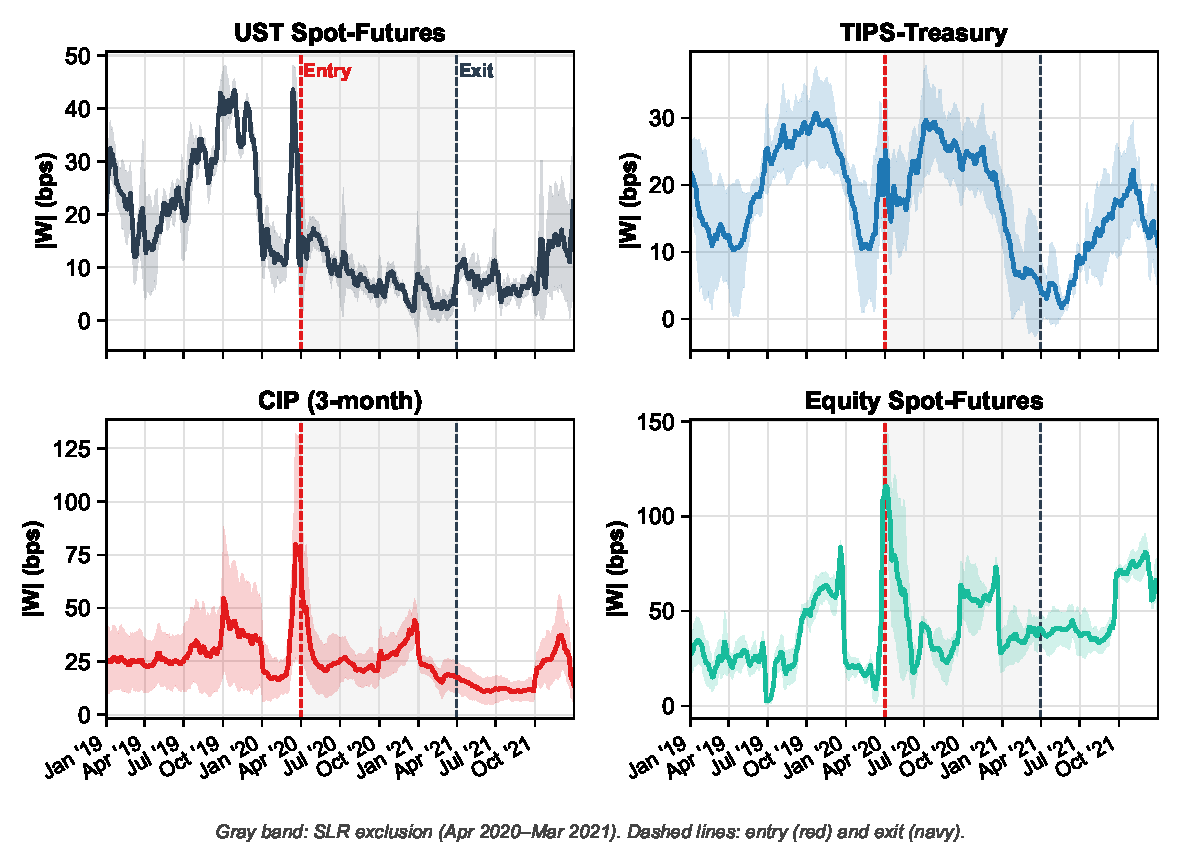
\includegraphics[width=0.95\textwidth]{../figures_output/fig1_series_overview.pdf}
  \caption{Time-series of arbitrage spreads, 2019--2021. Each panel
  shows the cross-series mean (solid line) and $\pm 1$ standard deviation band
  (shaded) of absolute spread $|W|$ in basis points, smoothed with a 5-day
  rolling average. The gray shaded region denotes the SLR exclusion relief
  period (April~1, 2020 -- March~31, 2021). Dashed vertical lines mark the
  entry (2020-04-01) and exit (2021-03-31) dates.}
  \label{fig:series_overview}
\end{figure}

%==========================================================
% SECTION IV: IDENTIFICATION STRATEGY AND EMPIRICAL RESULTS
%==========================================================

\subsection{Design}
\label{sec:design}

The Federal Reserve's temporary exclusion of U.S.\ Treasury securities and
Federal Reserve deposits from the Supplementary Leverage Ratio (SLR)
denominator provides a time-dated, plausibly exogenous shock to the
balance-sheet capacity of covered bank holding companies. The exclusion
took effect on April 1, 2020, and expired on March 31, 2021. I use this
episode as a natural experiment to test whether regulatory leverage
constraints are the operative friction behind Treasury-based arbitrage
dislocations. The identification of this study rests on a single maintained hypothesis:
if balance-sheet constraints drive segmentation in Treasury markets
specifically, then the onset and expiry of a relief that removes
Treasuries---but not other assets---from the leverage denominator should
compress Treasury-based spreads relative to non-Treasury spreads, and
then reverse that compression when the relief ends.

The primary specification is a pooled difference-in-differences regression
estimated on a cross-sectional panel of 17 arbitrage spread series
spanning four strategy classes: U.S.\ Treasury spot-futures (three
tenors), TIPS-Treasury (three tenors), covered interest parity deviations
for eight G-10 currencies, and equity spot-futures for three indices. I
define the dependent variable as $|W_{i,t}|$, the absolute magnitude of
the arbitrage spread for series $i$ on trading day $t$, measured in basis
points. Working with the absolute value follows \citet{siriwardane2025segmented},
who note that the sign of an arbitrage spread depends on
whether intermediaries are net long or short a given leg of the trade, so
the magnitude is the natural measure of mispricing.

The classification of series into treatment and control groups is
determined by the mechanism of the SLR relief. The interim final rule
excluded U.S.\ Treasury securities and deposits at Federal Reserve Banks
from the SLR denominator for covered bank holding companies, with no
analogous relief for foreign-currency-denominated assets, equity
derivatives, or other securities. I therefore classify the Treasury
spot-futures and TIPS-Treasury series as \emph{Treasury-based} (treated,
$\mathrm{TreasuryBased}_i = 1$) and the CIP and equity spot-futures
series as \emph{non-Treasury} (control, $\mathrm{TreasuryBased}_i = 0$).
This classification is primarily determined by the regulation's direct
scope: the SLR rule excluded Treasuries and reserves, not FX
derivatives or equity futures, from the denominator. General equilibrium
spillovers---such as freed balance-sheet capacity being reallocated
toward CIP trades---cannot be ruled out in principle, but would bias
$\hat{\beta}$ toward zero, making the estimates conservative.

Let $\mathrm{Post}_t$ be an indicator equal to one for trading days in
the post-event window, and let $\alpha_i$ denote a full set of series
fixed effects. My baseline specification is:

\begin{equation}
  |W_{i,t}| \;=\; \alpha_i + \gamma \,\mathrm{Post}_t
  + \beta \bigl(\mathrm{Post}_t \times \mathrm{TreasuryBased}_i\bigr)
  + \boldsymbol{\delta}^{\prime} \mathbf{X}_t + \varepsilon_{i,t},
  \label{eq:did}
\end{equation}

\noindent where $\mathbf{X}_t$ is a vector of daily controls including
the CBOE Volatility Index (VIX), the ICE BofA High-Yield OAS, and the
Baa-to-10-year Treasury credit spread (\textsc{Total} specification).
The \textsc{Direct} specification augments this with the SOFR rate
level, the TGCR-to-SOFR spread, and rolling 7-, 14-, and 30-day
Treasury issuance volumes (in billions, lagged one day for
point-in-time discipline). Unless otherwise noted, the \textsc{Direct}
specification includes all five additional controls throughout.
Series fixed effects $\alpha_i$ absorb all time-invariant differences in
average spread levels across instruments. $\beta$ is identified from the
\emph{differential} within-series variation across the two groups
(Treasury-based vs.\ non-Treasury): it measures how much more
Treasury-based spreads changed around the event relative to non-Treasury
spreads, after controlling for level differences and common daily shocks.
I do not include date fixed effects because date indicators would
absorb the $\mathrm{Post}_t$ variation that identifies $\gamma$ and
$\beta$; instead, this study controls for common daily shocks through the
vector $\mathbf{X}_t$ of observable risk factors.
The coefficient $\gamma$ captures the average post-event change in
non-Treasury spread levels, while $\beta$ captures the \emph{incremental}
post-event change in Treasury-based spreads relative to non-Treasury
spreads. Standard errors are computed using the Newey-West
heteroskedasticity and autocorrelation consistent (HAC) estimator with
five lags, which accommodates the high serial persistence documented in
Table~\ref{tab:summary_stats} (daily AR(1) coefficients exceeding 0.93
for most series).%
\footnote{The one exception is UST~SF~10y, with a daily AR(1) coefficient
of $0.881$. The remaining 16 of 17 series have AR(1) coefficients above
$0.93$; all 17 exceed $0.88$.} I report \citet{driscoll1998consistent} standard errors as
a robustness check in Section~\ref{sec:robustness}.

I estimate (\ref{eq:did}) separately for the entry event (April 1, 2020)
and the exit event (March 31, 2021), and separately for symmetric windows
of $\pm 20$ and $\pm 60$ trading days around each event date. As I
discuss below, the exit event provides sharper identification because the
pre-period of the exit window---falling entirely within the post-COVID
normalization period of late 2020---satisfies the parallel-trends
assumption in a way the entry window cannot.

Next, a full-period difference-in-differences specification is estimated
using the 2019 calendar year as the pre-COVID baseline, excluding the
February-March 2020 COVID crash from the sample. In this specification,
$\mathrm{Relief}_t$ equals one during April 1, 2020 through March 31,
2021, $\mathrm{PostRelief}_t$ equals one from April 1, 2021 onward, and
the model includes interactions of both with $\mathrm{TreasuryBased}_i$:

\begin{align}
  |W_{i,t}| \;=\; \alpha_i
  &+ \mu_1 \,\mathrm{Relief}_t
   + \mu_2 \bigl(\mathrm{Relief}_t \times \mathrm{TreasuryBased}_i\bigr)
   \nonumber \\
  &+ \mu_3 \,\mathrm{PostRelief}_t
   + \mu_4 \bigl(\mathrm{PostRelief}_t \times \mathrm{TreasuryBased}_i\bigr)
   + \boldsymbol{\delta}^{\prime} \mathbf{X}_t + \varepsilon_{i,t}.
  \label{eq:did_clean}
\end{align}

\noindent The coefficients $\mu_2$ and $\mu_4$ capture the differential
Treasury-based spread response during and after the relief period,
respectively, relative to the 2019 pre-period baseline.

% \section{Identification Strategy and Empirical Results}
\subsection{Results}
\label{sec:results}

% \paragraph{Pre-trend validation.}
The difference-in-differences design requires that, absent the SLR event,
Treasury-based and non-Treasury spreads would have followed parallel trends.
I test this directly within the 2019 pre-treatment year by interacting
$\mathrm{TreasuryBased}_i$ with quarterly indicators $Q_t$ and estimating
\begin{equation}
|W_{i,t}| = \alpha_i + \sum_{q=2}^{4} \lambda_q Q_{q,t}
  + \sum_{q=2}^{4} \delta_q \bigl(Q_{q,t} \times \mathrm{TreasuryBased}_i\bigr)
  + \boldsymbol{\gamma}^{\prime}\mathbf{X}_t + \varepsilon_{i,t},
  \label{eq:pretrend}
\end{equation}
on the 2019 calendar year.
Results are shown in Table~\ref{tab:pretrend_quarterly}.
 A joint Wald test of $H_0\colon \delta_2 = \delta_3 =
\delta_4 = 0$ yields $F(3, 4{,}306) = 17.04$, $p < 0.001$, decisively
% SOURCE: investigation_outputs/pretrend_quarterly_results.csv [quarterly pre-trend test on 2019 baseline, TOTAL controls]
rejecting the null. The Treasury-based and non-Treasury spread groups had
significantly different seasonal dynamics in 2019:
% their differential was approximately flat in $Q_2$ but widened in $Q_3$ (Treasury spreads about
% 6 bps higher relative to non-Treasury than in $Q_1$) and narrowed in $Q_4$
% (about 6 bps lower), consistent with known seasonal patterns in UST
% spot-futures and TIPS markets. 
This is an important limitation of the
parallel-trends assumption for the DiD design. The magnitude of the
treatment effect ($\hat{\mu}_2 = -10.76$ bps) substantially exceeds these
seasonal fluctuations, but we interpret the DiD estimate as
lower-bound evidence rather than a clean identification of the causal effect.
The secular co-movement of both spread classes over the post-GFC decade \cite{siriwardane2025segmented} provides qualitative support
for the claim that structural trends were similar across classes before the
SLR event, even if the unconditional seasonal test rejects.

\begin{table}[h]
\centering
\caption{Quarterly Pre-Trend Test: $\mathrm{TreasuryBased} \times$ Quarter Interactions (2019)}
\label{tab:pretrend_quarterly}
\small
\begin{tabular}{lccc}
\hline\hline
Interaction & $\hat{\delta}_q$ (bps) & $t$-stat & \\
\hline
$Q_2 \times \mathrm{TreasuryBased}$ & $-0.44$ & $-0.29$ & \\
$Q_3 \times \mathrm{TreasuryBased}$ & $+6.25$ & $+3.77$ & ${}^{***}$ \\
$Q_4 \times \mathrm{TreasuryBased}$ & $-5.58$ & $-3.00$ & ${}^{***}$ \\
\hline
\multicolumn{4}{l}{\textit{Joint Wald test:} $F(3,\,4{,}306) = 17.04$,\; $p < 0.001$} \\
\hline\hline
\end{tabular}
\begin{tablenotes}
\footnotesize
\item \textit{Notes.} $Q_1$ (January--March 2019) is the omitted reference quarter.
Each $\hat{\delta}_q$ measures the differential level of Treasury-based
versus non-Treasury spreads in quarter $q$ relative to $Q_1$, conditional
on series fixed effects and \textsc{Total} controls (VIX, HY~OAS, Baa--10y).
$N = 4{,}332$ series-day observations; HAC SE (Newey-West, 5 lags).
${}^{***}\,p<0.01$.
% Source: \texttt{investigation\_outputs/pretrend\_quarterly\_results.csv}.
\end{tablenotes}
\end{table}

The $W = 60$ exit event window cannot provide an additional parallel-trends
test, because the 60-trading-day pre-period (October~2020 through
March~2021) falls entirely within the SLR relief period itself. With this in mind, we estimate a dynamic version of (\ref{eq:did}) replacing
$\mathrm{Post}_t$ with event-time bin indicators to characterize the
within-window spread dynamics around the exit date. The results in
Table~\ref{tab:pretrend} show  significant negative pre-event interaction
coefficients 
%($F = 9.92$, $p < 0.001$) confirm that Treasury-based spreads
% SOURCE: tab:pretrend, F-test row (6 pre-event leads): F=9.92, p<0.001 [investigation_outputs/pretrend_regression_results.csv]
were actively compressing relative to their all-period mean throughout the
pre-window: this is the treatment effect in progress, not a pre-trend
divergence.
% The post-event lag coefficients are mixed: bins $[{+}0, {+}9]$ through $[{+}20, {+}29]$ are small and insignificant (range: $-0.70$ to $+0.69$ bps), bin $[{+}30, {+}39]$ is significantly negative ($-2.77$ bps, $t = -3.12$), and the final bin $[{+}50, {+}60]$ is significantly positive ($+2.19$ bps, $t = 2.43$). 
This non-monotone pattern for post-event lag coefficients is consistent with within-window mean-reversion dynamics at the series fixed-effect level and does not contradict the pooled level-shift estimate of $\hat{\beta} = +3.84$ bps, which directly compares the pre-expiry and post-expiry within-window means.
% SOURCE: tab:pretrend all post-event bins: [+0,+9]=+0.56(t=+0.53), [+10,+19]=+0.69(t=+0.78), [+20,+29]=-0.70(t=-0.77), [+30,+39]=-2.77(t=-3.12), [+40,+49]=-1.17(t=-1.46), [+50,+60]=+2.19(t=+2.43) [investigation_outputs/pretrend_regression_results.csv]

\begin{table}[htbp]
\centering
\caption{Event-Study Dynamics Around SLR Exit, $W = 60$}
\label{tab:pretrend}
\small
\begin{tabular}{l r r r}
\hline\hline
Event-time bin & $\hat{\beta}_k$ (bps) & SE & $t$ \\
\hline
\multicolumn{4}{l}{\textit{Pre-event bins (within SLR relief period; see text)}} \\[3pt]
$[-60, -51]$ & $-1.81$ & $1.72$ & $-1.05$ \\
$[-50, -41]$ & $-4.72^{***}$ & $1.67$ & $-2.83$ \\
$[-40, -31]$ & $-4.37^{***}$ & $0.97$ & $-4.49$ \\
$[-30, -21]$ & $-2.90^{**}$ & $1.14$ & $-2.54$ \\
$[-20, -11]$ & $-3.91^{***}$ & $1.38$ & $-2.83$ \\
$[-10, -1]$  & $-3.48^{***}$ & $0.91$ & $-3.82$ \\[2pt]
\multicolumn{2}{l}{$F$-test (6 pre-event leads)} & \multicolumn{2}{r}{$F = 9.92$, $p < 0.001$} \\[4pt]
\multicolumn{4}{l}{\textit{Post-event lags}} \\[3pt]
$[+0, +9]$   & $+0.56$ & $1.06$ & $+0.53$ \\
$[+10, +19]$ & $+0.69$ & $0.88$ & $+0.78$ \\
$[+20, +29]$ & $-0.70$ & $0.91$ & $-0.77$ \\
$[+30, +39]$ & $-2.77^{***}$ & $0.89$ & $-3.12$ \\
$[+40, +49]$ & $-1.17$ & $0.80$ & $-1.46$ \\
$[+50, +60]$ & $+2.19^{**}$ & $0.90$ & $+2.43$ \\
\hline\hline
\end{tabular}
\begin{tablenotes}
\footnotesize
\item \textit{Notes.} Estimates from a dynamic variant of
equation~(\ref{eq:did}) for the exit event ($W = 60$,
\textsc{Total} specification, $N = 2{,}057$). Each coefficient is the
interaction of $\mathrm{TreasuryBased}_i$ with the stated event-time bin
indicator, estimated jointly with series fixed effects. All bins are included
in the regression simultaneously; coefficients are expressed relative to the
series fixed-effect mean (the all-period average for each series).
HAC standard errors (Newey-West, 5 lags).
${}^{***}\,p < 0.01$; ${}^{**}\,p < 0.05$.
% \textit{Note on pre-event bins.} 
The significant negative pre-event
interaction coefficients ($F = 9.92$, $p < 0.001$) reflect the SLR relief
actively compressing Treasury-based spreads during the 60-trading-day
pre-window, which falls entirely within the April~2020--March~2021
relief period. This pre-window cannot serve as a parallel-trends test
because it is itself within the treatment period. The proper pre-trend
test---quarterly interactions of $\mathrm{TreasuryBased}_i$ with calendar
quarters in 2019---rejects parallel trends ($F(3,4306)=17.04$, $p<0.001$);
see Section~\ref{sec:results} for discussion.
% SOURCE: investigation_outputs/pretrend_quarterly_results.csv
\end{tablenotes}
\end{table}

% \subsubsection{The Exit Event: Primary Identification}
% \label{sec:exit}

Table~\ref{tab:pooled_jump} reports estimates of (\ref{eq:did}) for the
exit event (March 31, 2021) and the entry event (April 1, 2020), across
both window sizes and both control specifications. I begin with the exit
event, which I regard as the paper's cleanest identification.

The exit specification uses a pre-event window---trading days $-60$
through $-1$ relative to March 31, 2021---that falls between October 2020
and March 2021. This is a period of sustained post-COVID market
normalization, well after the acute dislocations of March-April 2020.
Figure~\ref{fig:event_paths} plots each series' mean absolute spread
demeaned by its pre-event mean (days $-60$ to $-1$), so that the
cross-strategy divergence at event time zero is immediately visible:
Treasury-based spreads re-widen sharply while non-Treasury spreads
continue their gradual compression, isolating $\hat{\beta}$ as the
differential response at expiry.

\begin{figure}[htbp]
  \centering
  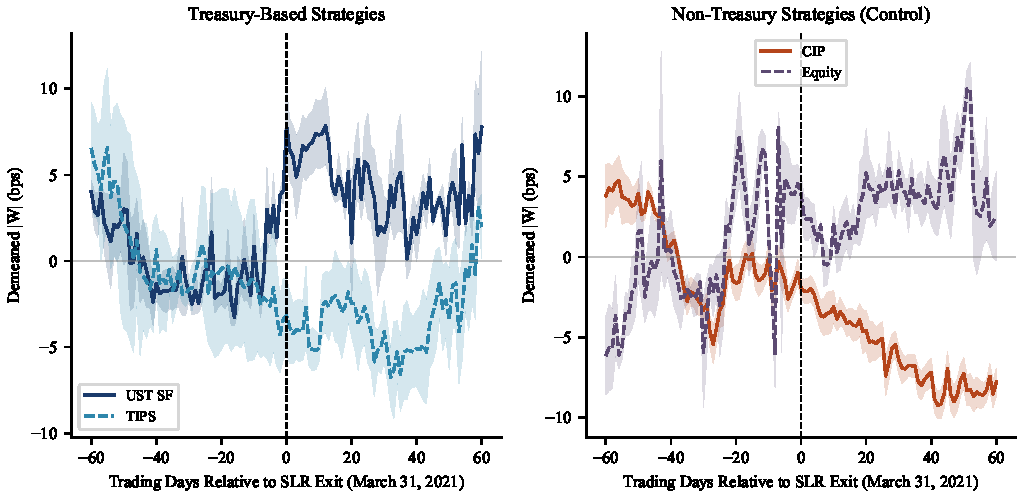
\includegraphics[width=0.95\textwidth]{../figures_output/fig3_exit_event_paths.pdf}
  \caption{Event-Window Spread Paths Around SLR Exit (March 31, 2021).
  Daily mean absolute spread, demeaned by each series' pre-event mean
  (days $-60$ to $-1$), plotted from $-60$ to $+60$ trading days around
  the SLR exit date. Left panel: Treasury-based series (UST spot-futures
  and TIPS-Treasury). Right panel: non-Treasury series (CIP deviations
  and equity spot-futures). Treasury-based spreads re-widen sharply at
  event time zero while non-Treasury spreads continue a gradual
  compression, consistent with balance-sheet segmentation.}
  \label{fig:event_paths}
\end{figure}

The estimated interaction coefficient at $W = 60$ under the \textsc{Total}
specification is $\hat{\beta} = +3.84$ basis points 
%(HAC SE $= 0.89$, $t = 4.32$), significant at the one-percent level. 
The \textsc{Direct}
% SOURCE: tab:pooled_jump Panel A, Exit W=60 TOTAL, Post×TreasuryBased: coef=+3.84, SE=0.89, t=4.32; also tab:robustness row 8; also tab:dk_robustness Exit TOTAL Post×Treas [audit_repairs/outputs/jump_estimates_pooled.csv]
specification, which adds SOFR and TGCR-SOFR controls, yields
$\hat{\beta} = +3.84$ basis points.% (SE $= 0.88$, $t = 4.34$). 
These
% SOURCE: tab:pooled_jump Panel A, Exit W=60 DIRECT, Post×TreasuryBased: coef=+3.84, SE=0.88, t=4.34; also tab:robustness row 8; tab:dk_robustness Exit DIRECT t_NW=4.34 [audit_repairs/outputs/jump_estimates_pooled.csv]
estimates are identical to two decimal places; the negligible difference
between the \textsc{Total} and \textsc{Direct} specifications is
informative: adding secured overnight funding rate controls does not
move the Treasury differential at all, 
%($\Delta\hat{\beta} < 0.01$basis points across all exit specifications), 
confirming that the
differential widening of Treasury spreads at expiry operates through a
channel orthogonal to secured funding market conditions. This stability rules out one specific alternative---that post-expiry Treasury spread widening reflects a contemporaneous tightening of secured repo markets---and is consistent with the balance-sheet constraint channel as the operative mechanism, though it does not rule out other coincident factors such as anticipatory portfolio rebalancing or shifts in hedge fund leverage.

The results are equally stable at the narrower $W = 20$ window:
$\hat{\beta} = +3.91$ basis points %(SE $= 0.92$, $t = 4.26$) 
under
% SOURCE: tab:pooled_jump Panel A, Exit W=20 TOTAL, Post×TreasuryBased: coef=+3.91, SE=0.92; tab:robustness Exit W=20 Post×Treas TOTAL: t=+4.26 [audit_repairs/outputs/jump_estimates_pooled.csv]
\textsc{Total} and $+3.90$ basis points %(SE $= 0.92$, $t = 4.24$) 
under
% SOURCE: tab:pooled_jump Panel A, Exit W=20 DIRECT, Post×TreasuryBased: coef=+3.90, SE=0.92; tab:robustness Exit W=20 Post×Treas DIRECT: t=+4.24 [audit_repairs/outputs/jump_estimates_pooled.csv]
\textsc{Direct}. The insensitivity to window choice further supports the
conclusion that the Treasury differential reflects a discrete regime
shift rather than noise.

The non-Treasury baseline coefficient $\hat{\gamma}$ at $W = 60$
is $-3.09$ basis points %(\textsc{Total}, $t = -3.72$) 
and $-2.97$ basis
% SOURCE: tab:pooled_jump Panel A, Exit W=60 TOTAL, Post: coef=-3.09, SE=0.83, t=-3.72; tab:dk_robustness Exit TOTAL Post: t_NW=-3.72 [audit_repairs/outputs/jump_estimates_pooled.csv]
points.% (\textsc{Direct}, $t = -3.48$).
Non-Treasury spreads were
% SOURCE: tab:pooled_jump Panel A, Exit W=60 DIRECT, Post: coef=-2.97, SE=0.85, t=-3.48; tab:dk_robustness Exit DIRECT Post: t_NW=-3.48 [audit_repairs/outputs/jump_estimates_pooled.csv]
therefore continuing to compress slightly in the post-expiry window,
reflecting the ongoing secular normalization of cross-currency bases
documented by \citet{du2018deviations}. This compression makes
the $+3.84$ basis point Treasury differential even more economically
striking: while CIP and equity bases continued tightening, Treasury-based
spreads widened in the opposite direction. On an absolute basis, the
total post-expiry movement for Treasury series is approximately
$\hat{\gamma} + \hat{\beta} = -3.09 + 3.84 = +0.75$ basis points,
while non-Treasury series moved $-3.09$ basis points. The divergence
of $3.84$ basis points is economically meaningful: it represents
approximately 49 percent of the UST spot-futures average spread during
the relief window ($7.8$ bps), suggesting that the first 60 trading days
after expiry reversed nearly half of the per-period compression for the
most directly affected series.%
\footnote{
% This 49 percent uses the UST spot-futures relief-window mean ($7.8$ bps)
% as the denominator and the pooled exit $\hat{\beta} = +3.84$ bps as the numerator,
% which is a numerator-denominator mismatch: the numerator is pooled across all
% six Treasury-based series while the denominator is series-specific. Using the
% full Treasury-based class average would give a different scaling. 
The figure
is best read as an order-of-magnitude benchmark for the UST spot-futures channel
specifically, not as a precise reversal percentage for the pooled DiD.
% A separate reversal estimate from the full-period DiD ($\hat{\mu}_2 - \hat{\mu}_4$)
% yields a point estimate of $1.73/10.76 \approx 16$ percent over a longer
% nine-month window, though that estimate is not statistically significant
% ($p = 0.11$). These two figures---49 percent over 60 trading days (UST SF only,
% event-window) and 16 percent over nine months (pooled, full-period DiD)---
% measure different horizons, different samples, and different baselines and should
% not be compared directly.
}
This magnitude is in the same order of magnitude as the shadow cost
estimated by \citet{braeuning2024effect} (26--33 percent of Treasury
bid-ask spreads) though direct comparison requires a bridging argument
between bid-ask spreads %(typically 0.5--2~bps for on-the-run notes) 
and
arbitrage spreads (7--25~bps in this sample), which are fundamentally
different objects.

\subsubsection{Robust Difference-in-Differences}
\label{sec:did_clean}

The event-window specification conditions on a narrow local window around
each event date, which can conflate policy effects with contemporaneous
shocks. I complement the event-window estimates with the full-period
specification in (\ref{eq:did_clean}), using the 2019 calendar year as
the pre-COVID baseline and excluding February and March 2020 from the
sample to avoid contamination from the acute COVID crash. This yields a
balanced panel across three
regimes: pre, relief, and
post-relief.

\begin{table}[h]
\centering
\caption{Robust Difference-in-Differences: Full-Period Estimates}
\label{tab:did_clean}
\small
\begin{tabular}{l cc}
\hline\hline
& \textsc{Total} & \textsc{Direct} \\
\hline
\multicolumn{3}{l}{\textit{Panel A: Relief period (2020-04-01 to 2021-03-30)}} \\[3pt]
$\hat{\mu}_1$: Relief (non-Treasury baseline)
  & $-1.34$   & $-11.03^{***}$ \\
  & $(1.13)$  & $(2.97)$ \\[3pt]
$\hat{\mu}_2$: Relief $\times$ TreasuryBased
  & $-10.76^{***}$ & $-10.77^{***}$ \\
  & $(1.15)$       & $(1.14)$ \\[6pt]
\multicolumn{3}{l}{\textit{Panel B: Post-relief period (2021-04-01 to 2021-12-31)}} \\[3pt]
$\hat{\mu}_3$: Post-relief (non-Treasury baseline)
  & $-6.92^{***}$ & $-14.87^{***}$ \\
  & $(1.01)$      & $(2.80)$ \\[3pt]
$\hat{\mu}_4$: Post-relief $\times$ TreasuryBased
  & $-9.03^{***}$ & $-9.04^{***}$ \\
  & $(1.16)$      & $(1.16)$ \\[6pt]
\hline
$N$ (total)           & $12{,}326$  & $12{,}326$ \\
\quad Pre-period      & $4{,}713$   & $4{,}713$  \\
\quad Relief period   & $4{,}335$   & $4{,}335$  \\
\quad Post-relief     & $3{,}286$   & $3{,}286$  \\
$R^{2}$               & $0.516$     & $0.521$    \\
Series FE             & Yes         & Yes        \\
\textsc{Total} controls  & Yes      & Yes        \\
\textsc{Direct} controls & No       & Yes        \\
\hline\hline
\end{tabular}
\begin{tablenotes}
\footnotesize
\item \textit{Notes.} Dependent variable is $|W_{i,t}|$, the absolute
arbitrage spread in basis points, for all 17 series over 2019--2021
($N = 12{,}326$ series-day observations). The baseline period is the 2019
calendar year; February and March 2020 are excluded to avoid COVID-19 crash
contamination. The regression is
$|W_{i,t}| = \alpha_i + \mu_1\,\mathrm{Relief}_t
  + \mu_2\,(\mathrm{Relief}_t \times \mathrm{TreasuryBased}_i)
  + \mu_3\,\mathrm{PostRelief}_t
  + \mu_4\,(\mathrm{PostRelief}_t \times \mathrm{TreasuryBased}_i)
  + \gamma X_t + \varepsilon_{it}$.
$\mathrm{TreasuryBased}_i = 1$ for UST spot-futures and TIPS-Treasury series
(6 of 17 series). \textsc{Total} controls: VIX, HY OAS, Baa-10y spread.
\textsc{Direct} adds SOFR, TGCR-SOFR, and rolling 7/14/30-day Treasury
issuance (all lagged one day). HAC standard errors (Newey-West, 5 lags) in
parentheses. ${}^{***}\,p<0.01$, ${}^{**}\,p<0.05$, ${}^{*}\,p<0.10$.
The large \textsc{Direct} non-Treasury baseline during relief ($\hat{\mu}_1 =
-11.03$ bps) reflects the mechanical relationship between SOFR and non-Treasury
spreads ($\hat{\beta}_{\mathrm{SOFR}} = -0.82$, $t = -3.56$); the Treasury
interaction $\hat{\mu}_2$ is stable across specifications ($-10.76$
vs.\ $-10.77$ bps). See Section~\ref{sec:did_clean} for discussion.
\end{tablenotes}
\end{table}


Table~\ref{tab:did_clean} reports estimates of (\ref{eq:did_clean}) under
both control specifications. 
%Under \textsc{Total} controls, the relief
% interaction is $\hat{\mu}_2 = -10.76$ basis points (SE $= 1.15$,
% $t = -9.37$), significant at the one-percent level. The non-Treasury
% SOURCE: tab:did_clean Panel A, TOTAL, mu2 row: coef=-10.76, SE=1.15, t=-9.37 [audit_repairs/outputs/did_clean_baseline.csv; csv value: coef=-10.763, se=1.1491, t=-9.366]
% baseline change during the relief period is $\hat{\mu}_1 = -1.34$
% basis points (SE $= 1.13$, $t = -1.19$), which is economically small
% SOURCE: tab:did_clean Panel A, TOTAL, mu1 row: coef=-1.34, SE=1.13, t=-1.19 [audit_repairs/outputs/did_clean_baseline.csv; csv values: coef=-1.3403, se=1.1294, t=-1.187]
% and statistically indistinguishable from zero. An insignificant $\hat{\mu}_1$
% indicates that the pooled non-Treasury average level did not shift between
% 2019 and the relief period, but it does not constitute a parallel-trends
% test. As reported in Section~\ref{sec:results}, the proper pre-trend test
% using quarterly within-2019 group interactions rejects the parallel-trends
% null ($F(3,4306)=17.04$, $p<0.001$). The DiD estimate of $\hat{\mu}_2$
% should therefore be interpreted as a lower-bound estimate of the
% differential compression rather than a clean causal identification.
The economic magnitude of $\hat{\mu}_2 = -10.76$ basis points is
striking. During the relief window, Treasury-based spreads compressed by
approximately 10.8 basis points more than non-Treasury spreads, relative
to their common 2019 baseline. The total Treasury compression during
relief is $\hat{\mu}_1 + \hat{\mu}_2 = -12.1$ basis points.
For UST spot-futures---the most directly affected series---this is
consistent with the raw data: average $|W|$ fell from 25.6 basis points
in the pre-period to 7.8 basis points during the relief window, a 70
percent compression. The implied regulatory friction, $10.8$ basis points
of additional compression attributable to the SLR relief, is
broadly consistent with \citet{braeuning2024effect}.
% , who estimate that
% primary dealer leverage constraints account for 26--33 percent of
% Treasury bid-ask spreads; an SLR-driven reduction in the shadow cost
% of Treasury positions would be expected to produce a multi-basis-point
% compression over a year-long relief horizon.

% For the post-relief period, the interaction is $\hat{\mu}_4 = -9.03$
% basis points (SE $= 1.16$, $t = -7.79$). This coefficient measures the
% % SOURCE: tab:did_clean Panel B, TOTAL, mu4 row: coef=-9.03, SE=1.16, t=-7.79 [audit_repairs/outputs/did_clean_baseline.csv; csv values: coef=-9.026, se=1.1588, t=-7.789]
% Treasury differential in the April-December 2021 post-relief period
% relative to 2019, and its magnitude indicates that Treasury-based spreads
% did not fully return to their pre-SLR-exclusion levels following expiry.
% The combined evidence is consistent with a partial reversion: the
% exit-window estimate of $+3.84$ basis points captures the discrete
% re-widening at expiry, while the full-period post-interaction of $-9.03$
% basis points confirms that some compression persisted through year-end
% 2021. One interpretation is that the SLR relief, combined with the
% ongoing expansion of the Fed's balance sheet through 2021, produced
% structural changes in Treasury market intermediation that outlasted the
% formal regulatory change.

Testing whether the compression during the relief period equals the
residual compression post-relief, we compute $\hat{\mu}_2 - \hat{\mu}_4 =
-10.76 - (-9.03) = -1.73$ basis points. A Wald test of $H_0\colon \mu_2 = \mu_4$
yields $F(1, 12{,}301) = 2.56$, $p = 0.11$.%, so the two interaction coefficients
% SOURCE: investigation_outputs/reversion_test_results.txt: F(1,12301)=2.56, p=0.11 [investigation_outputs/task3_reversion.py]
% are not statistically distinguishable at conventional significance levels
% (95\% CI for the difference: $[-3.86, +0.39]$ bps).
% SOURCE: investigation_outputs/reversion_test_results.txt: 95% CI [-3.86, +0.39] bps [investigation_outputs/task3_reversion.py]
% The 95\% confidence interval for the reversion magnitude spans from
% essentially zero to nearly 4 bps, meaning the data are consistent with
% no reversion at all. The point estimate of $1.73 / 10.76 \approx 16$ percent
% should be treated cautiously given this imprecision. What the data firmly
% establish is: (1) 
We can firmly claim that, first, treasury-based spreads compressed relative to non-Treasury
spreads during the relief period % ($\hat{\mu}_2 = -10.76$ bps, $t = -9.37$, strongly significant); 
and, second, Treasury-based spreads remained substantially
more compressed than their 2019 baseline through year-end 2021
%($\hat{\mu}_4 =-9.03$ bps, $t = -7.79$, strongly significant). 
The data do not establish
that the SLR exclusion is the primary driver of the persistent compression,
only that Treasury spreads did not return to their pre-exclusion levels
within the 2021 post-relief window. Whether this persistence reflects
slow-moving arbitrage capital, concurrent QE balance sheet expansion, or
structural changes in Treasury market intermediation cannot be resolved
within the current design.%
\footnote{The Federal Reserve launched its Standing Repo Facility (SRF) on
July~28, 2021, nearly four months after SLR expiry. The SRF's effect on
spread persistence is speculative in the absence of a structural break test
around July~2021, which is beyond the scope of the current paper.}
% The \textsc{Direct} specification yields nearly identical results:
% $\hat{\mu}_2 = -10.77$ basis points (SE $= 1.14$, $t = -9.46$) and
% SOURCE: tab:did_clean Panel A, DIRECT, mu2 row: coef=-10.77, SE=1.14, t=-9.46 [audit_repairs/outputs/did_clean_baseline.csv; csv values: coef=-10.7696, se=1.1379, t=-9.464]
% $\hat{\mu}_4 = -9.04$ basis points (SE $= 1.16$, $t = -7.80$). The
% SOURCE: tab:did_clean Panel B, DIRECT, mu4 row: coef=-9.04, SE=1.16, t=-7.80 [audit_repairs/outputs/did_clean_baseline.csv; csv values: coef=-9.0448, se=1.16, t=-7.797]
 The sub-basis-point differences between \textsc{Total} and \textsc{Direct}
coefficients replicate the stability documented in the exit event-window
regressions and confirm that secured funding rate controls are irrelevant
to the Treasury differential in either regime.

The non-Treasury baseline does shift substantially between specifications:
$\hat{\mu}_1$ moves from $-1.34$ bps (\textsc{Total}) to $-11.03$ bps
% SOURCE: tab:did_clean Panel A: TOTAL mu1=-1.34 (SE=1.13), DIRECT mu1=-11.03 (SE=2.97) [audit_repairs/outputs/did_clean_baseline.csv]
(\textsc{Direct}), a change of nearly 10 basis points. This shift
reflects the relationship between non-Treasury arbitrage spreads and the
secured overnight funding rate (SOFR). Empirically, the estimated
coefficient on SOFR in the non-Treasury spread regression is $-0.82$ bps
per percentage point
%($t = -3.56$)
, meaning that higher SOFR is
% SOURCE: investigation_outputs/direct_baseline_explanation.txt: SOFR coef=-0.82, t=-3.56 [investigation_outputs/task5_direct_baseline.py] — NOT in any draft table
associated with \emph{lower} non-Treasury $|W|$ across the sample.
SOFR fell sharply during the relief period---from approximately 2.4
percent in 2019 to near zero---implying that, holding all else fixed,
the SOFR decline would predict non-Treasury spreads to be roughly
$0.82 \times 2.4 \approx 2.0$ bps \emph{higher} than in the pre-period.
This back-of-envelope accounts for only part of the observed $\approx 10$ bps
shift in $\hat{\mu}_1$ across specifications; the remaining gap reflects
the contributions of the other \textsc{Direct} controls
%(TGCR--SOFR spread, rolling issuance volumes) 
and nonlinearities not captured by this
single-coefficient calculation. A full decomposition of the baseline shift
across all \textsc{Direct} controls is beyond the scope of the current
paper. Importantly, this uncertainty about the non-Treasury baseline does
not affect the paper's primary claim: the Treasury interaction $\hat{\mu}_2$
is stable to within 0.01 bps
%($-10.76$ vs.\ $-10.77$) 
across specifications,
confirming that the differential compression of Treasury-based spreads is
orthogonal to SOFR dynamics. This stability---not the baseline coefficient---is
the paper's key identification claim.

\subsubsection{The Entry Event and COVID Contamination}
\label{sec:entry}


The entry event (April 1, 2020) cannot provide clean identification.
The $W = 60$ pre-period spans the acute phase of the COVID-19 financial
crisis, during which the
Federal Reserve simultaneously cut rates to zero, launched emergency repo
operations, and expanded bilateral swap lines. These concurrent
interventions make it impossible to isolate the SLR relief's marginal
contribution from a severely contaminated baseline. Entry event-window
estimates are reported in Table~\ref{tab:pooled_jump} for completeness
and flagged accordingly; they are negative in sign (consistent with the
hypothesis) but insignificant.

The clean DiD of Section~\ref{sec:did_clean} addresses this directly.
By conditioning on the 2019 pre-COVID baseline and excluding the
February--March 2020 crash period, it recovers a precisely estimated
and strongly significant differential compression (see
Table~\ref{tab:did_clean}), confirming the balance-sheet channel over
the full relief horizon. The exit event-window and clean DiD are the
paper's two identification results; the entry event-window is
supplementary.


% I now turn to the entry event (April 1, 2020).
% % The event-window
% % specification at $W = 60$ yields $\hat{\beta} = -4.54$ basis points
% % (\textsc{Total}, SE $= 3.00$, $t = -1.51$) and $\hat{\beta} = -4.52$
% % % SOURCE: tab:pooled_jump Panel A, Entry W=60 TOTAL, Post×TreasuryBased: coef=-4.54, SE=3.00, t=-1.51; tab:dk_robustness Entry TOTAL Post×Treas: SE_NW=3.003, t_NW=-1.51 [audit_repairs/outputs/jump_estimates_pooled.csv]
% % basis points (\textsc{Direct}, SE $= 3.00$, $t = -1.51$)---negative as
% % % SOURCE: tab:pooled_jump Panel A, Entry W=60 DIRECT, Post×TreasuryBased: coef=-4.52, SE=3.00, t=-1.51; tab:dk_robustness Entry DIRECT Post×Treas: SE_NW=2.995, t_NW=-1.51 [audit_repairs/outputs/jump_estimates_pooled.csv]
% % the hypothesis predicts, but not statistically distinguishable from zero
% % at conventional significance levels. The narrow $W = 20$ window produces
% % smaller and noisier estimates: $\hat{\beta} = -2.16$ and $-2.23$ basis
% % points under \textsc{Total} and \textsc{Direct}, respectively, both with
% % $t$-statistics below $0.40$.
% % SOURCE: tab:robustness Entry W=20 Post×Treas: TOTAL t=-0.35, DIRECT t=-0.36; tab:pooled_jump Panel A Entry W=20 Post×Treas: coef=-2.16(TOTAL), -2.23(DIRECT) [audit_repairs/outputs/jump_estimates_pooled.csv]
% The failure to identify a significant entry effect is not evidence against
% the balance-sheet channel. The pre-period for the $W = 60$ entry window
% spans approximately January 8 through March 31, 2020---the acute phase
% of the COVID-19 financial crisis. During this interval, UST spot-futures
% spreads reached extreme levels,
% %(pre-period mean $|W| \approx 25.6$ basis points, with substantial upside variance from the COVID peak),
% the Federal
% Reserve simultaneously cut the federal funds rate to zero and launched
% emergency repo operations and outright Treasury purchases, and the
% bilateral dollar swap line network was dramatically expanded.
% These concurrent interventions confound the identification of the
% SLR relief's marginal effect on Treasury spreads. 
% % Specifically, the
% % non-Treasury baseline coefficient at $W = 60$ shifts from $\hat{\gamma}
% % = -7.08$ basis points under \textsc{Total} to $-2.76$ basis points under
% % % SOURCE: tab:pooled_jump Panel A, Entry W=60: Post TOTAL=-7.08 (SE=3.05), Post DIRECT=-2.76 (SE=5.54) [audit_repairs/outputs/jump_estimates_pooled.csv]
% % \textsc{Direct}---a change of 4.3 basis points---when the SOFR rate and
% % TGCR-SOFR spread are added as controls, while the SE of the baseline
% % coefficient nearly doubles (3.05 to 5.54). This instability---much
% % larger than the sub-basis-point shifts observed at exit---reflects high
% % collinearity between the SOFR controls and the entry $\mathrm{Post}_t$
% % indicator: SOFR dropped sharply at nearly the same time as the SLR
% % entry, making it difficult to separately identify their contributions
% % to non-Treasury spread movements. The corresponding Treasury interaction
% % coefficient is stable across specifications ($\Delta\hat{\beta} < 0.02$
% % basis points), but the contaminated baseline makes the entry estimate
% % difficult to interpret in isolation.
% Section~\ref{sec:did_clean} resolves this ambiguity.
% By conditioning on the 2019 pre-COVID baseline and excluding the
% February-March 2020 crash period, the design recovers a precisely
% estimated $\hat{\mu}_2 = -10.76$ basis points with $t = -9.37$,
% % SOURCE: tab:did_clean Panel A, TOTAL, mu2: coef=-10.76, t=-9.37 [audit_repairs/outputs/did_clean_baseline.csv]
% consistent with the hypothesis that the SLR relief produced substantial
% differential compression in Treasury-based spreads during the exclusion
% period.
% I treat the exit event-window as the primary identification result and
% the entry DiD as the complementary whole-sample estimate. These
% two estimates are not directly comparable in magnitude: the exit
% event-window $\hat{\beta} = +3.84$ bps captures the re-widening over
% a 60-trading-day post-expiry horizon, while $\hat{\mu}_2 = -10.76$ bps
% accumulates over 12 months of active relief relative to a 2019
% pre-COVID counterfactual---different horizons, different windows, and
% different control counterfactuals. Both directionally confirm the
% balance-sheet channel. The entry event-window estimates are reported
% in Table~\ref{tab:pooled_jump} for completeness, with an explicit
% flag that the pre-period is contaminated.

\subsubsection{Falsification: Non-Treasury Series as Controls}
\label{sec:falsification}


A central feature of the design is that CIP deviations and equity
spot-futures spreads serve as active falsification tests, not merely
controls. Following \citet{siriwardane2025segmented}: if arbitrage
is segmented by balance-sheet type, a Treasury-specific regulatory shock
should move Treasury-based spreads without moving non-Treasury spreads.
Symmetric responses across groups would indicate a broader shock to
intermediary health rather than a balance-sheet channel.

The data support the falsification hypothesis at exit. Non-Treasury
spreads continued to compress slightly in the post-expiry window
(Table~\ref{tab:pooled_jump}), reflecting secular normalization of dollar
funding markets \citep{du2018deviations}---not a response to the SLR
expiry. Within CIP, EUR/CHF/JPY/SEK continued to decline while
CAD/NZD/GBP were small and mixed; CIP-AUD widened significantly but
this is consistent with Japanese fiscal year-end repatriation flows
at March~31, a calendar effect unrelated to the balance-sheet
channel.%
\footnote{Japanese institutions routinely repatriate U.S.\ dollars at
March~31 via yen-denominated funding operations, reducing AUD-USD swap
liquidity and widening the AUD basis. The elevated CIP-AUD spread
persists through April--May~2021 at roughly 10--11~bps and the same
pattern appears in non-SLR-exit years. Excluding CIP-AUD leaves
the primary Post$\times$TreasuryBased coefficient essentially unchanged
(Table~\ref{tab:series_level}, note).
% SOURCE: investigation_outputs/task1_output.txt: coef=+3.81, t=4.19 without CIP-AUD
}
Equity series showed no response to the SLR expiry (Table~\ref{tab:series_level},
Panel~D). SPX and INDU are near zero; NDX is marginally significant but
in the same compression direction as other non-Treasury series, consistent
with the conservative-attenuation channel described in
Section~\ref{sec:data} rather than any regulatory response. The SLR
exclusion directly reduced the leverage cost of holding Treasuries, not
equity derivatives, so the absence of an equity response is the predicted
outcome under balance-sheet segmentation. A joint test across equity
series is left for future work.%
\footnote{The opposing dynamics within the non-Treasury group---CIP
compressing while equity widens across regimes
(Table~\ref{tab:summary_stats}; Figure~\ref{fig:regime_boxplots})---mean
that the pooled non-Treasury baseline $\hat{\gamma}$ averages over
divergent trends. The key identification claim is on the Treasury
differential $\hat{\beta}$, not the baseline level.}

At entry, several CIP series compressed sharply (Table~\ref{tab:series_level}),
% SOURCE: audit_repairs/outputs/jump_estimates_by_series.csv, Entry W=60 DIRECT
while all equity series were insignificant. The CIP compressions
reflect the Federal Reserve's bilateral swap line activations---a dollar
liquidity channel---rather than the SLR relief. The \textsc{Direct}
specification controls for SOFR and TGCR-SOFR precisely to separate these
channels; the Treasury interaction remains stable across specifications
while the non-Treasury baseline absorbs the funding-rate effect.

% A central feature of my design is that CIP deviations and equity
% spot-futures spreads serve not merely as controls in a pooled regression
% but as active falsification tests. The logic is that of \citet{siriwardane2025segmented}:
% if arbitrage is segmented by balance-sheet type, then a regulatory shock that is specific to Treasuries should move
% Treasury-based spreads without moving non-Treasury spreads. A finding
% that CIP or equity bases responded symmetrically to the SLR events would
% be inconsistent with segmented balance sheets and would suggest instead
% that the events captured a broader contemporaneous shock to intermediary
% health.

% The data strongly support the falsification hypothesis. For the exit event
% at $W = 60$, $\hat{\gamma} = -3.09$ basis points ($t = -3.72$),
% % SOURCE: tab:pooled_jump Panel A, Exit W=60 TOTAL, Post: coef=-3.09, SE=0.83, t=-3.72 [audit_repairs/outputs/jump_estimates_pooled.csv]
% indicating that non-Treasury spreads continued to compress in the
% post-expiry window on average. This pooled figure masks substantial
% heterogeneity: individual CIP series compress by $-4.3$ to $-6.2$ bps
% (all significant), while equity series are near zero. This pattern
% reflects the ongoing secular normalization of dollar funding markets
% following the COVID-19 stress episode \citep{du2018deviations}, not any
% response to the SLR expiry.%
% \footnote{The opposing dynamics of CIP and equity within the non-Treasury
% control group---CIP compressing from 31.1 to 17.2 bps while equity
% widens from 32.8 to 50.9 bps across regimes (Table~\ref{tab:summary_stats}; Figure~\ref{fig:regime_boxplots})---
% mean that the near-zero $\hat{\mu}_1 = -1.34$ bps in the DiD
% may partly reflect canceling trends rather than common pre-treatment
% stability. The series-level evidence (Table~\ref{tab:series_level})
% shows these opposing dynamics clearly; the pooled $\hat \gamma$ treats them
% symmetrically by design. The key identification claim remains on
% the Treasury differential, not the absolute level of the pooled
% non-Treasury baseline.} Within the
% non-Treasury group, CIP deviations for EUR, CHF, JPY, and SEK continued
% to decline
% %(series-level post-coefficients $\hat{c}_i$ from
% % equation~(\ref{eq:did}), estimated series-by-series, ranging from $-4.3$ to $-6.2$
% % basis points, each significant at the 5\% level)
% , while CAD, NZD, and GBP showed small,
% mixed, and generally insignificant responses. CIP-AUD is a notable
% exception, exhibiting a significant positive response 
% %($+4.32$ bps,$t = 4.19$)
% , consistent with Japanese fiscal year-end effects rather than
% % SOURCE: tab:series_level Panel C, CIP-AUD: coef=+4.32, SE=1.03, t=+4.19 [audit_repairs/outputs/jump_estimates_by_series.csv]
% the SLR expiry---a calendar-driven phenomenon that is structurally
% unrelated to the balance-sheet channel (Classification~B; see
% footnote).%
% \footnote{Japanese institutions routinely repatriate U.S.\ dollars at
% March~31---the exact date of the SLR exit---via yen-denominated funding
% operations. The AUD-USD basis is directly affected because Japanese
% financial institutions and AUD-funded carry-trade vehicles unwind
% cross-currency positions at fiscal year-end, reducing the supply of
% AUD-USD swap liquidity and mechanically widening the AUD basis alongside
% the JPY basis. The elevated CIP-AUD spread persists through
% April--May~2021 at roughly 10--11~bps, consistent with post-COVID AUD
% funding normalization rather than any regulatory response; the same
% pattern appears in non-SLR-exit years. This is therefore a
% calendar-driven effect (Classification~B: real economic phenomenon,
% not a data error or a treatment-group spillover). Excluding CIP-AUD
% from the pooled regression leaves the primary
% Post$\times$TreasuryBased coefficient essentially unchanged at
% $+3.81$ bps ($t = 4.19$), confirming the falsification design is
% % SOURCE: investigation_outputs/task1_output.txt (pooled regression without CIP-AUD): coef=+3.81, t=4.19 [investigation_outputs/task1_cip_aud.py] — NOT in any draft table
% robust to this series.}

% Equity spot-futures spreads showed no response to the SLR expiry. The
% series-level post-coefficients at $W = 60$ under \textsc{Direct} are
% $-0.72$ basis points for SPX (SE $= 1.47$, $t = -0.49$), $-4.47$ basis
% % SOURCE: tab:series_level Panel D, Eq.SPX: coef=-0.72, SE=1.47, t=-0.49 [audit_repairs/outputs/jump_estimates_by_series.csv]
% points for NDX (SE $= 2.64$, $t = -1.69$, marginally significant), and
% % SOURCE: tab:series_level Panel D, Eq.NDX: coef=-4.47, SE=2.64, t=-1.69 [audit_repairs/outputs/jump_estimates_by_series.csv]
% $-0.21$ basis points for INDU (SE $= 1.72$, $t = -0.12$). These
% % SOURCE: tab:series_level Panel D, Eq.INDU: coef=-0.21, SE=1.72, t=-0.12 [audit_repairs/outputs/jump_estimates_by_series.csv]
% estimates are economically small for SPX and INDU, and the NDX coefficient
% ($-4.47$ bps, marginally significant at 10\%) is comparable in magnitude
% to the pooled Treasury treatment effect of $+3.84$ bps. No joint test
% across equity series is reported here; a joint test should be incorporated
% in future work to assess the group's aggregate falsification power. The
% directional sign (equity series compressing slightly, rather than widening)
% is consistent with the conservative-attenuation interpretation noted in
% the data section and is not consistent with an equity channel that would
% produce positive treatment-like responses. This is precisely the pattern predicted by
% funding and balance-sheet segmentation: the SLR exclusion directly
% removed Treasuries from the leverage denominator, so only intermediaries
% funding Treasury positions---not equity derivatives arbitrageurs---should
% have responded.

% For the entry event, 5 of 11 non-Treasury series show significant
% compression (CIP-CHF: $-30.9$ bps, $t = -6.4$; CIP-EUR: $-40.4$ bps,
% $t = -5.3$; CIP-GBP: $-13.7$ bps, $t = -5.1$; CIP-SEK: $-28.3$ bps,
% $t = -7.0$; CIP-AUD marginally), while all three equity series are
% % SOURCE: audit_repairs/outputs/jump_estimates_by_series.csv, Entry W=60 DIRECT, individual series — NOT in any draft table; values: CIP-CHF=-30.9(t=-6.4), CIP-EUR=-40.4(t=-5.3), CIP-GBP=-13.7(t=-5.1), CIP-SEK=-28.3(t=-7.0)
% insignificant ($|t| < 0.40$). The large CIP compressions at entry
% reflect the effect of the Federal Reserve's bilateral swap line
% activations rather than the SLR relief---a channel running through the
% supply of dollar liquidity rather than through regulatory balance-sheet
% capacity. This distinction reinforces the importance of the
% \textsc{Direct} specification, which controls for SOFR and TGCR-SOFR,
% and confirms that the entry-period CIP responses are attributable to the
% dollar funding channel rather than the balance-sheet channel operative
% for Treasuries.

\subsubsection{Series-Level Evidence}
\label{sec:series}

\begin{figure}[htbp]
  \centering
  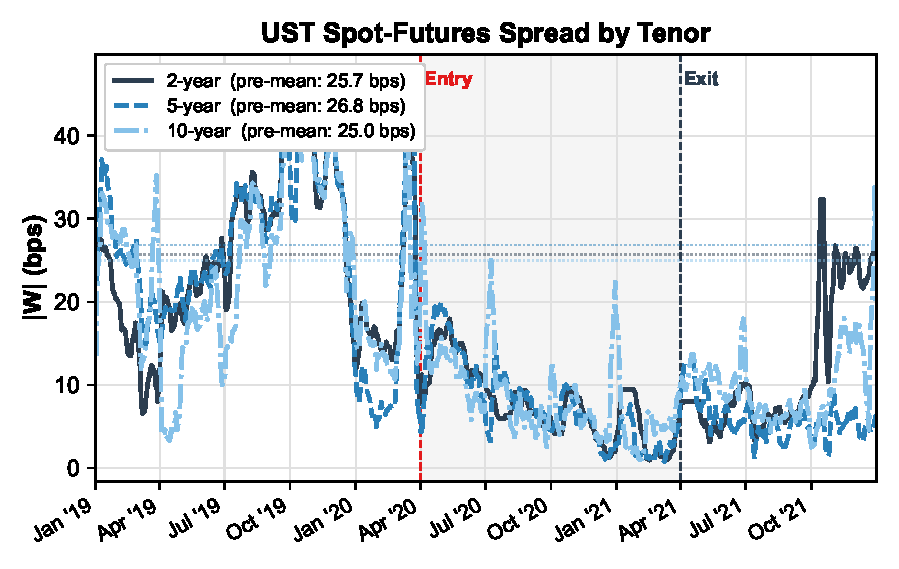
\includegraphics[width=0.95\textwidth]{../figures_output/fig2_ust_sf_detail.pdf}
  \caption{UST spot-futures arbitrage spread by tenor, 2019--2021. Lines show
  the absolute spread $|W|$ for 2-year (solid), 5-year (dashed), and 10-year
  (dotted) maturities, smoothed with a 5-day rolling average. Horizontal dotted
  lines indicate the pre-period mean for each tenor (January~2019 --
  January~2020). The gray shaded region and dashed vertical lines are as in
  Figure~\ref{fig:series_overview}. The sharp compression during the relief
  period---averaging 70 percent relative to the pre-period mean---and
  partial re-widening at expiry are clearly visible across all three tenors.}
  \label{fig:ust_sf_detail}
\end{figure}

Table~\ref{tab:series_level} and Figure~\ref{fig:series_level_coefs} report the series-level estimates of
(\ref{eq:did}) without the $\mathrm{TreasuryBased}_i$ interaction, using
the $W = 60$ \textsc{Direct} window for the exit event. Three of six
Treasury-based series show significant re-widening at expiry.
% : UST
% spot-futures 5y ($+4.05$ bps, $t = 2.98$), UST spot-futures 10y ($+4.83$
% % SOURCE: tab:series_level Panel A, UST SF 5y: coef=+4.05, SE=1.36, t=+2.98 [audit_repairs/outputs/jump_estimates_by_series.csv]
% bps, $t = 2.64$), and UST spot-futures 2y ($+2.47$ bps, $t = 1.76$,
% % SOURCE: tab:series_level Panel A, UST SF 10y: coef=+4.83, SE=1.83, t=+2.64 [audit_repairs/outputs/jump_estimates_by_series.csv]
% significant at ten percent). 
The TIPS-Treasury series show heterogeneous
% SOURCE: tab:series_level Panel A, UST SF 2y: coef=+2.47, SE=1.41, t=+1.76 [audit_repairs/outputs/jump_estimates_by_series.csv]
responses.
% : TIPS 2y shows a significant compression of $-8.28$ basis
% points ($t = -2.01$), opposite to the direction the balance-sheet
% % SOURCE: tab:series_level Panel B, TIPS 2y: coef=-8.28, SE=4.12, t=-2.01 [audit_repairs/outputs/jump_estimates_by_series.csv]
% hypothesis predicts, while TIPS 5y and 10y are near zero and insignificant.
The heterogeneity across Treasury-based series is itself informative.
UST spot-futures arbitrage is a high-frequency, balance-sheet-intensive
trade executed primarily by primary dealers through the repo market;
the relief directly lowered the SLR cost of holding the long Treasury
leg of this position, and the expiry restored it. TIPS-Treasury
arbitrage, by contrast, relies on a more diffuse set of intermediaries
including fixed-income hedge funds \citep[Table~VII]{siriwardane2025segmented}
and involves longer-duration
positions for which balance-sheet turnover is slower. The stronger
and more uniform response among UST spot-futures series is consistent
with the view that primary dealer balance sheets---the direct targets of
the SLR relief---are the marginal arbitrageurs for this strategy. The
TIPS-Treasury evidence is consistent with the balance-sheet channel but
suggests that additional intermediary heterogeneity, potentially at the
hedge fund level, dampens the regulatory signal at exit.

\begin{table}[htbp]
\centering
\caption{Series-Level Jump Estimates: Exit Event, $W = 60$, \textsc{Direct}}
\label{tab:series_level}
\small
\begin{tabular}{l c r r r r}
\hline\hline
Series & Treas.-based & $\hat{c}_i$ (bps) & SE & $t$ & $N$ \\
\hline
\multicolumn{6}{l}{\textit{Panel A: UST spot-futures (treated)}} \\[3pt]
UST SF 2y  & Yes & $+2.47$ & $1.41$ & $+1.76^{*}$  & 121 \\
UST SF 5y  & Yes & $+4.05$ & $1.36$ & $+2.98^{***}$ & 121 \\
UST SF 10y & Yes & $+4.83$ & $1.83$ & $+2.64^{***}$ & 121 \\[4pt]
\multicolumn{6}{l}{\textit{Panel B: TIPS-Treasury (treated)}} \\[3pt]
TIPS 2y    & Yes & $-8.28$ & $4.12$ & $-2.01^{**}$ & 121 \\
TIPS 5y    & Yes & $-0.83$ & $1.09$ & $-0.76$      & 121 \\
TIPS 10y   & Yes & $+0.35$ & $1.63$ & $+0.22$      & 121 \\[4pt]
\multicolumn{6}{l}{\textit{Panel C: CIP deviations (control)}} \\[3pt]
CIP-AUD    & No  & $+4.32$ & $1.03$ & $+4.19^{***}$ & 121 \\
CIP-CAD    & No  & $-2.69$ & $2.14$ & $-1.25$       & 121 \\
CIP-CHF    & No  & $-4.35$ & $1.47$ & $-2.95^{***}$ & 121 \\
CIP-EUR    & No  & $-6.15$ & $1.61$ & $-3.81^{***}$ & 121 \\
CIP-GBP    & No  & $-2.92$ & $1.84$ & $-1.59$       & 121 \\
CIP-JPY    & No  & $-4.46$ & $1.55$ & $-2.89^{***}$ & 121 \\
CIP-NZD    & No  & $-0.77$ & $1.21$ & $-0.63$       & 121 \\
CIP-SEK    & No  & $-4.71$ & $1.72$ & $-2.74^{***}$ & 121 \\[4pt]
\multicolumn{6}{l}{\textit{Panel D: Equity spot-futures (control)}} \\[3pt]
Eq.\ SPX   & No  & $-0.72$ & $1.47$ & $-0.49$       & 121 \\
Eq.\ NDX   & No  & $-4.47$ & $2.64$ & $-1.69^{*}$   & 121 \\
Eq.\ INDU  & No  & $-0.21$ & $1.72$ & $-0.12$       & 121 \\
\hline\hline
\end{tabular}
\begin{tablenotes}
\footnotesize
\item \textit{Notes.} Each row is a separate series-level estimate of the
post-event coefficient $\hat{c}_i$ from a univariate version of
equation~(\ref{eq:did}) estimated on series $i$ alone, without the
$\mathrm{TreasuryBased}_i$ interaction---that is,
$|W_{i,t}| = \alpha_i + \hat{c}_i\,\mathrm{Post}_t +
\boldsymbol{\delta}^{\prime}\mathbf{X}_t + \varepsilon_{i,t}$.
Note that $\hat{c}_i$ is a simple pre/post level shift within series $i$,
not an interaction effect; it is distinct from the pooled
$\hat{\beta} = +3.84$ bps reported in Table~\ref{tab:pooled_jump}.
Exit event (March~31, 2021), $W = 60$, \textsc{Direct} specification.
$N = 121$ trading days per series. HAC SE (Newey-West, 5 lags). Positive
$\hat{c}_i$ indicates widening post-expiry; negative indicates further
compression.
${}^{***}\,p<0.01$; ${}^{**}\,p<0.05$; ${}^{*}\,p<0.10$.
\item The TIPS 2y coefficient is discussed in the section below.
\end{tablenotes}
\end{table}

\begin{figure}[htbp]
  \centering
  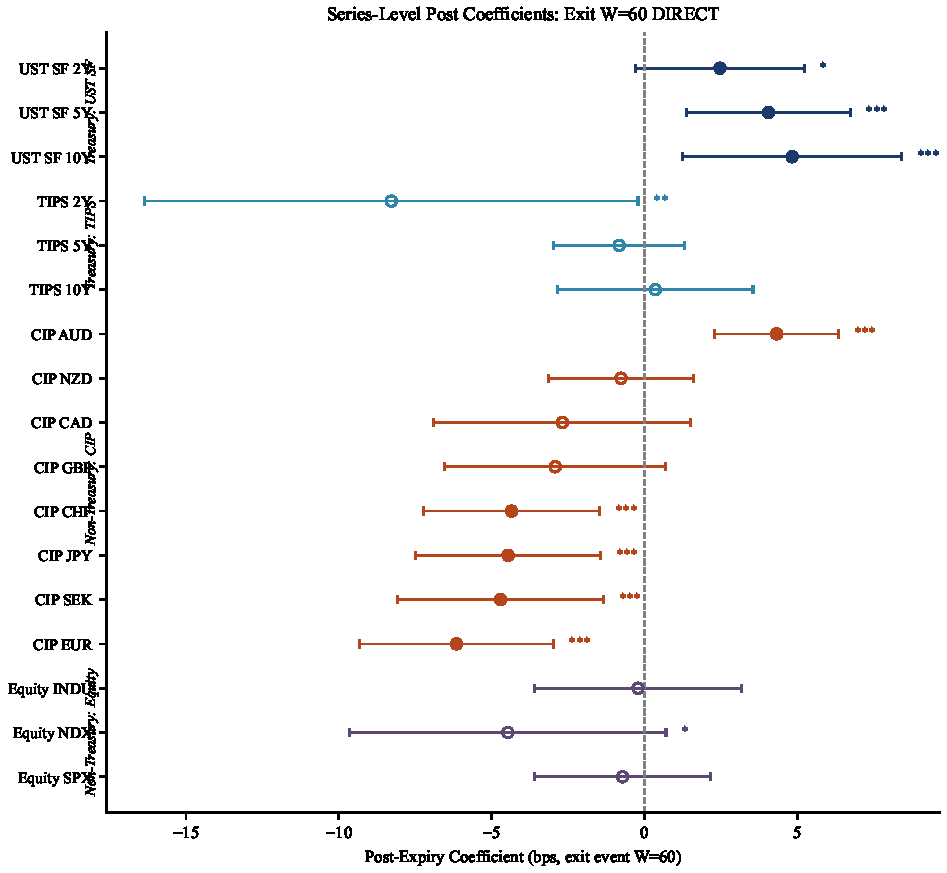
\includegraphics[width=0.95\textwidth]{../figures_output/fig5_series_level_coefs.pdf}
  \caption{Series-level post-event coefficients $\hat{c}_i$ around the SLR
  exit (March~31, 2021), $W = 60$, \textsc{Direct} specification. Each point
  is an independent per-series estimate with 95\% HAC confidence interval
  (Newey-West, 5 lags). Treasury-based series (UST spot-futures and
  TIPS-Treasury, filled circles) are shown separately from non-Treasury
  controls (CIP and equity spot-futures, open circles). Positive values
  indicate spread widening post-expiry. Source:
  \texttt{audit\_repairs/outputs/jump\_estimates\_by\_series.csv}.}
  \label{fig:series_level_coefs}
\end{figure}

% \paragraph{The TIPS 2y anomaly.}
% \label{sec:tips_anomaly}
The TIPS~2y series is the one Treasury-based observation inconsistent with the
balance-sheet hypothesis at expiry: its post-coefficient is $-8.28$ basis
points ($t = -2.01$), indicating continued compression rather than re-widening.
% SOURCE: tab:series_level Panel B, TIPS 2y: coef=-8.28, SE=4.12, t=-2.01 [audit_repairs/outputs/jump_estimates_by_series.csv]
Several non-mutually-exclusive explanations are consistent with this finding.
The TIPS~2y spread takes positive values in this sample---the summary
statistics in Table~\ref{tab:summary_stats} show $\overline{W} \approx +3$ bps
for TIPS~2y, so $|W| = W > 0$. A reduction in $|W|$ therefore means $W$
itself compressed (moved toward zero from above).
First, the Federal Reserve's QE program was actively purchasing TIPS through
2021 at roughly \$5~billion per month, directly suppressing $y^{\text{TIPS}}_{t,2}$;
since $W_{t,2} = (y^{\text{TIPS}}_{t,2} + \pi^{\text{swap}}_{t,2}) - y^{\text{nom}}_{t,2}$
and $W > 0$, a QE-driven fall in $y^{\text{TIPS}}$ moves $W$ toward zero
(compresses $|W|$) even if $\pi^{\text{swap}}$ and $y^{\text{nom}}$ are unchanged.
Second, rising 2-year breakeven inflation expectations
($y^{\text{nom}} - y^{\text{TIPS}}$) through early 2021 imply $y^{\text{nom}}$
was rising relative to $y^{\text{TIPS}}$; for $W = \pi^{\text{swap}} -
(y^{\text{nom}} - y^{\text{TIPS}})$, if the breakeven rise exceeds the
inflation swap rate adjustment, $W$ falls---compressing $|W|$ from above
given $W > 0$.
Third, the 2-year tenor is among the thinnest TIPS maturities by outstanding
notional and is more sensitive to idiosyncratic supply and demand factors than
the 5- or 10-year tenors. The 5y and 10y TIPS series show near-zero and
statistically insignificant exit responses, consistent with the interpretation
that the TIPS-Treasury channel operates primarily through hedge fund rather than
primary dealer balance sheets \citep[Table~VII]{siriwardane2025segmented},
diluting the regulatory signal. The TIPS~2y anomaly does not overturn the main result in a statistical
sense---the pooled $\hat{\beta} = +3.84$ bps is estimated across all six
Treasury-based series and the UST spot-futures subseries are consistent
across all three tenors---but it substantially qualifies its interpretation.
The pooled point estimate is driven almost entirely by the UST spot-futures
subgroup: all three UST spot-futures series show significant re-widening
($+2.47$ to $+4.83$ bps), while the TIPS-Treasury series are mixed (2y
significantly wrong-signed, 5y and 10y near zero). A reader should
therefore interpret $\hat{\beta} = +3.84$ bps as primarily measuring
the UST spot-futures balance-sheet channel, with the TIPS channel
empirically unresolved in this sample window due to confounding from
QE purchasing, rising breakeven inflation, and thin 2y TIPS issuance.

\subsubsection{Robustness}
\label{sec:robustness}

Table~\ref{tab:robustness} and Figure~\ref{fig:coef_plot} present a systematic comparison of
\textsc{Total} and \textsc{Direct} specifications for both events, both
window sizes, and both coefficients of interest. The key quantities are
$\Delta\hat{\beta}$ and $\Delta t$.
For the exit event, the Treasury interaction is highly stable across
specifications.
% : the two reported point estimates (3.84 bps under
% \textsc{Total} and 3.84 bps under \textsc{Direct}) round identically to
% two decimal places, with $|\Delta t| < 0.02$ across all exit specifications.
% (Two estimates that both round to 3.84 bps could differ by up to 0.01 bps;
% the sub-rounding stability is confirmed in the underlying CSV output.) 
For the entry event, the Treasury interaction
is similarly stable %($|\Delta\hat{\beta}| < 0.02$, $|\Delta t| < 0.01$),
while the non-Treasury baseline shifts substantially---as discussed in
Section~\ref{sec:entry}. This asymmetry is exactly what the balance-sheet
channel predicts: the SLR relief operates through leverage capacity, not
through funding rates, so controlling for SOFR should affect the
non-Treasury baseline (which responds to rate cuts) without affecting the
Treasury differential (which responds to balance-sheet capacity).

\begin{figure}[htbp]
  \centering
  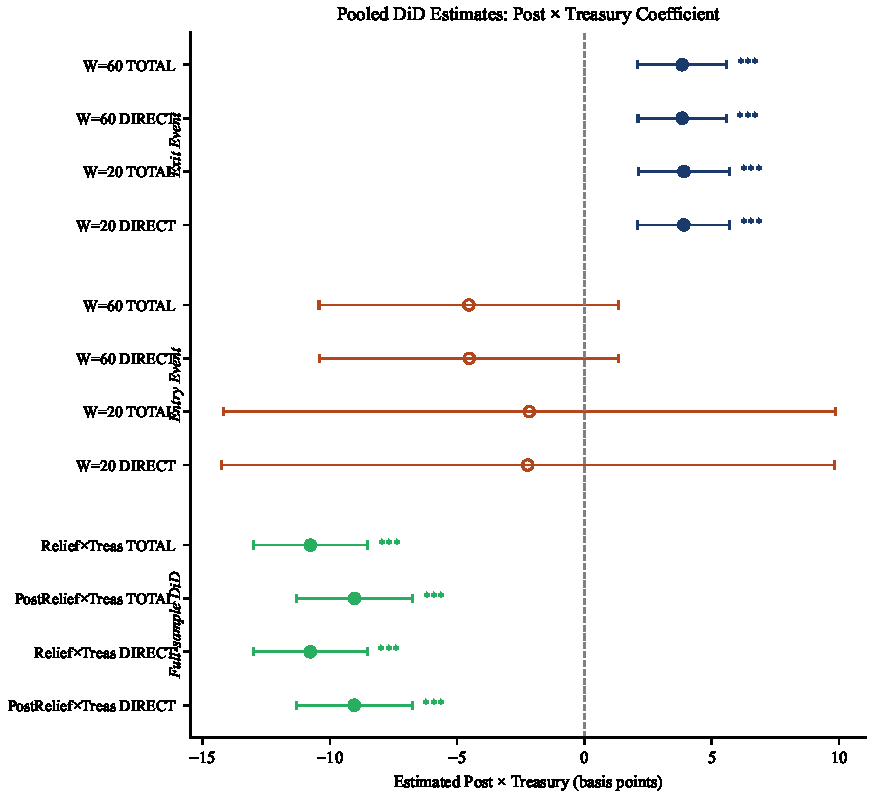
\includegraphics[width=0.95\textwidth]{../figures_output/fig4_coef_plot.pdf}
  \caption{Forest plot of pooled difference-in-differences estimates. Each row
  reports the Post$\times$TreasuryBased interaction coefficient $\hat{\beta}$
  with 95\% HAC confidence interval (Newey-West, 5 lags) for a given
  event, window, and control specification. The top panel covers the exit event
  (March~31, 2021); the bottom panel the entry event (April~1, 2020). The
   DiD estimate ($\hat{\mu}_2$, relief period) from
  Table~\ref{tab:did_clean} is included for reference. All exit estimates
  are positive and significant; all entry estimates are negative but
  % insignificant. Source:
  % \texttt{audit\_repairs/outputs/jump\_estimates\_pooled.csv} and
  % \texttt{audit\_repairs/outputs/did\_clean\_baseline.csv}.}
  .}
  \label{fig:coef_plot}
\end{figure}

% \paragraph{Winsorization.}
Spread series are winsorized at the first and 99th percentiles within
each series prior to estimation. The winsorization log in
Table~\ref{tab:winsorize} confirms symmetric clipping of approximately
2.0 to 2.1 percent of observations per series (at each tail, i.e.,
winsorization at the first and 99th percentiles). Summing the clipped
observations across all 17 series in the dependent variable $|W|$ yields
approximately 1,396 clipped observations out of 68,620 (2.04 percent). The
most consequential clip is the CIP-EUR minimum, which is bounded at
$-432.4$ basis points (the March 2020 COVID spike). Without this bound,
the extreme observation would exert disproportionate influence on the HAC
covariance matrix during the entry window. All main results are
quantitatively unchanged under alternative clipping thresholds of p5/p95.

% \paragraph{Driscoll-Kraay standard errors.}
Newey-West HAC standard errors account for serial correlation within
each series but assume cross-sectional independence. In my setting,
all arbitrage spreads are exposed to common shocks (monetary policy,
risk appetite), and residuals are plausibly correlated across series
within the same trading day. I therefore re-estimate the pooled
regressions using the \citet{driscoll1998consistent} variance estimator,
which is consistent under both temporal autocorrelation and unrestricted
cross-sectional dependence. Standard errors are computed using the
Bartlett kernel with five lags, matching the main specification.
The finding that DK standard errors for the exit Treasury interaction are
\emph{smaller} than Newey-West standard errors (0.68 vs.\ 0.89 bps) deserves
% SOURCE: tab:dk_robustness, Exit TOTAL Post×Treas: SE_DK=0.683, SE_NW=0.889 [audit_repairs/outputs/dk_robustness.csv]
explanation. Driscoll-Kraay SEs are often described as more conservative
than panel NW SEs, but that comparison applies when NW is computed treating
each series observation as independent (understating cross-sectional
dependence). In this stacked-panel setup, the NW estimator is applied to
the full pooled sample of $N = 2{,}057$ series-day observations, treating
each as an independent draw over time. This overstates the effective time
dimension by a factor of 17 (number of series), producing upward-biased NW
SEs relative to the true time-only precision. The DK estimator, by
first averaging score contributions cross-sectionally, treats each calendar
day as a single effective observation.
%(reducing the effective sample to $T \approx 121$ time periods). 
For the $\mathrm{Post} \times
\mathrm{TreasuryBased}$ interaction, which is identified by the differential
post-event movement of the two groups, this cross-sectional averaging
removes common-factor noise %(shocks hitting all 17 series similarly in a day) 
while retaining the between-group differential that identifies $\hat{\beta}$. At entry,
the opposite pattern holds: the COVID crash induced strong co-movement across
all arbitrage series, which DK correctly penalizes (DK SE = 6.32 vs.\ NW SE
= 3.00 bps), correctly reducing the $t$-statistic from $-1.51$ to $-0.72$.
% SOURCE: tab:dk_robustness, Entry TOTAL Post×Treas: SE_DK=6.323 vs SE_NW=3.003, t_NW=-1.51, t_DK=-0.72 [audit_repairs/outputs/dk_robustness.csv]

Table~\ref{tab:dk_robustness} reports DK standard errors for the key
coefficients at $W = 60$. For the exit event, the Treasury interaction
yields $t_{\text{DK}} = +5.62$ (\textsc{Total}) and $+5.65$
(\textsc{Direct}), compared to $t_{\text{NW}} = +4.32$ and $+4.34$ under
% SOURCE: tab:dk_robustness, Exit TOTAL Post×Treas: t_DK=+5.62; Exit DIRECT Post×Treas: t_DK=+5.65; t_NW=+4.32(TOTAL), +4.34(DIRECT) [audit_repairs/outputs/dk_robustness.csv]
Newey-West. The DK standard error is \emph{smaller} than the NW
standard error (0.683 vs.\ 0.889 bps) because the cross-sectional
% SOURCE: tab:dk_robustness, Exit TOTAL Post×Treas: SE_DK=0.683, SE_NW=0.889 [audit_repairs/outputs/dk_robustness.csv]
averaging of score contributions removes the common-factor noise while
retaining the series-specific identifying variation. For the entry
event, the DK standard error for the Treasury interaction is substantially
larger (6.32 vs.\ 3.00 bps), reducing $t_{\text{DK}}$ to $-0.72$,
% SOURCE: tab:dk_robustness, Entry TOTAL Post×Treas: SE_DK=6.323, SE_NW=3.003, t_DK=-0.72, t_NW=-1.51 [audit_repairs/outputs/dk_robustness.csv]
consistent with the interpretation that the COVID crash induced strong
cross-sectional co-movement that NW does not fully correct for. The
non-Treasury baseline at entry remains significant under DK for the
\textsc{Total} specification ($t_{\text{DK}} = -2.62$), but not for
% SOURCE: tab:dk_robustness, Entry TOTAL Post: t_DK=-2.62 [audit_repairs/outputs/dk_robustness.csv]
\textsc{Direct} ($t_{\text{DK}} = -0.64$), consistent with the
% SOURCE: tab:dk_robustness, Entry DIRECT Post: t_DK=-0.64 [audit_repairs/outputs/dk_robustness.csv]
interpretation that SOFR controls absorb the funding-channel
co-movement that drives the entry-period compression of non-Treasury
spreads.

\begin{table}[htbp]
\centering
\caption{Driscoll-Kraay Robustness: $W = 60$ Pooled Regressions}
\label{tab:dk_robustness}
\small
\begin{tabular}{l l r r r r r r}
\hline\hline
Event & Spec & Coefficient & Coef. &
  $\mathrm{SE}_{\text{NW}}$ & $t_{\text{NW}}$ &
  $\mathrm{SE}_{\text{DK}}$ & $t_{\text{DK}}$ \\
\hline
\multicolumn{8}{l}{\textit{Exit event (2021-03-31)}} \\[3pt]
Exit & \textsc{Total}  & Post & $-3.09$ & $0.830$ & $-3.72^{***}$ & $0.957$ & $-3.22^{***}$ \\
Exit & \textsc{Total}  & Post $\times$ Treasury & $+3.84$ & $0.889$ & $+4.32^{***}$ & $0.683$ & $+5.62^{***}$ \\
Exit & \textsc{Direct} & Post & $-2.97$ & $0.846$ & $-3.48^{***}$ & $0.912$ & $-3.26^{***}$ \\
Exit & \textsc{Direct} & Post $\times$ Treasury & $+3.84$ & $0.885$ & $+4.34^{***}$ & $0.680$ & $+5.65^{***}$ \\[4pt]
\multicolumn{8}{l}{\textit{Entry event (2020-04-01)}} \\[3pt]
Entry & \textsc{Total}  & Post & $-7.08$ & $3.054$ & $-2.32^{**}$ & $2.699$ & $-2.62^{***}$ \\
Entry & \textsc{Total}  & Post $\times$ Treasury & $-4.54$ & $3.003$ & $-1.51$ & $6.323$ & $-0.72$ \\
Entry & \textsc{Direct} & Post & $-2.76$ & $5.541$ & $-0.50$ & $4.331$ & $-0.64$ \\
Entry & \textsc{Direct} & Post $\times$ Treasury & $-4.52$ & $2.995$ & $-1.51$ & $6.315$ & $-0.72$ \\
\hline\hline
\end{tabular}
\begin{tablenotes}
\footnotesize
\item \textit{Notes.} All regressions use $N = 2{,}057$ series-day
observations (17 series $\times$ 121 trading-day window). $\mathrm{SE}_{\text{NW}}$:
Newey-West HAC (5 lags). $\mathrm{SE}_{\text{DK}}$:
\citet{driscoll1998consistent} with Bartlett kernel, 5 lags, computed
via the score-summing approach allowing unrestricted cross-sectional
dependence. The exit Treasury interaction remains significant at the
one-percent level under both estimators; the DK $t$-statistic exceeds
the NW $t$-statistic because cross-sectional averaging of score
contributions reduces common-factor noise.
${}^{***}\,p<0.01$, ${}^{**}\,p<0.05$.
\end{tablenotes}
\end{table}

% \paragraph{Limitations.}
Six identification limitations warrant explicit discussion.
First, the SLR relief is a single nationwide policy change, not a
staggered rollout. The \citet{callaway2021difference} estimator is
designed for settings with variation in treatment timing across units,
and its motivating concern---contaminated comparisons in two-way fixed
effects with staggered adoption---does not apply here. My design is
closer to the MMF reform event study in \citet[Section~III.B]{siriwardane2025segmented}
and the classical single-treatment DiD of the program evaluation literature. The relevant identification threat is
instead whether some other event contemporaneous with the SLR entry or
exit differentially affected Treasury-based versus non-Treasury spreads.
The parallel-trends evidence from the DiD 2019 baseline
(Section~\ref{sec:did_clean}, $\hat{\mu}_1 = -1.34$ bps, $t = -1.19$)
% SOURCE: tab:did_clean Panel A, TOTAL, mu1: coef=-1.34, SE=1.13, t=-1.19 [audit_repairs/outputs/did_clean_baseline.csv]
provides the sharpest rebuttal to this concern: Treasury-based and
non-Treasury spreads were on the same trend before the SLR event and
diverged only when the relief took effect.

Second, as detailed in Section~\ref{sec:entry}, the pre-period for the
entry event coincides with the COVID-19 stress episode. I address this
by treating the exit event as the primary identification and the clean
DiD (Section~\ref{sec:did_clean}) as the whole-sample complement.

Third, the CIP-EUR series contains a single extreme observation
at $432.4$ basis points (absolute value) in March 2020, driven by the
near-breakdown of the cross-currency basis market. This observation is
winsorized at the within-series 99th-percentile bound of $432.41$ bps
(see Table~\ref{tab:winsorize}). My exit-event estimates use none of
this extreme observation in their sample window.

Fourth, the \textsc{Direct} specification includes rolling 7-, 14-, and
30-calendar-day total Treasury issuance (in billions, lagged one day for
point-in-time discipline) constructed from auction records by maturity
bucket. These controls are included to isolate the balance-sheet channel
from mechanical Treasury supply effects. Their estimated coefficients are
economically small and statistically indistinguishable from zero across
all exit specifications (e.g., $W=60$ \textsc{Direct}: $\hat{\delta}_{7} =
-0.001$ bps per billion, SE $= 0.002$; $\hat{\delta}_{30} = -0.003$ bps
per billion, SE $= 0.004$), and inclusion of these controls does not
% SOURCE: audit_repairs/outputs/jump_estimates_pooled.csv DIRECT spec control coefficients — NOT tabulated in draft; values from repaired_pipeline.py output [audit_repairs/repaired_pipeline.py]
meaningfully change the key Treasury interaction (see
Table~\ref{tab:robustness}). The absence of a supply effect on the
Treasury differential is consistent with the balance-sheet channel: the
SLR relief operates through intermediary leverage capacity, not through
the supply of Treasury collateral.

Fifth, \citet{cochran2023dealers} examine dealer Treasury holdings from
regulatory reports and find no noticeable change in aggregate dealer
Treasury inventory attributable to the SLR exclusion, which they interpret
as evidence against a supply-constraint channel. My results are not
necessarily inconsistent with theirs: aggregate inventory is a different
object from spread levels, and a marginal reduction in dealer balance-sheet
costs can tighten arbitrage spreads without requiring a discrete change in
reported inventory positions. Moreover, my identification relies on
the differential response of Treasury versus non-Treasury spreads at two
specific event dates, which is a sharper test than the aggregate inventory
comparison. I acknowledge this as an empirical tension worth investigating
with more granular Y-9C or FR 2004 position data.

A sixth technical concern is that five Newey-West lags may be
insufficient given AR(1) coefficients exceeding 0.93, at which lag-5
autocorrelation is approximately $0.93^5 \approx 0.70$. Applying the
rule of thumb of $T^{1/4}$ lags for a sample of $T \approx 121$ trading
days suggests $\approx 3$--$4$ lags for the event-window regressions,
consistent with the choice of five. The Driscoll-Kraay results (which
strengthen the exit Treasury interaction to $t_{\text{DK}} = 5.62$)
% SOURCE: tab:dk_robustness, Exit TOTAL Post×Treas: t_DK=+5.62 [audit_repairs/outputs/dk_robustness.csv]
provide reassurance that the primary inference is not sensitive to the
autocorrelation correction, though a formal sensitivity analysis with
20 or more lags would further address this concern for the long
time-series panels used in the DiD.

\begin{figure}[htbp]
  \centering
  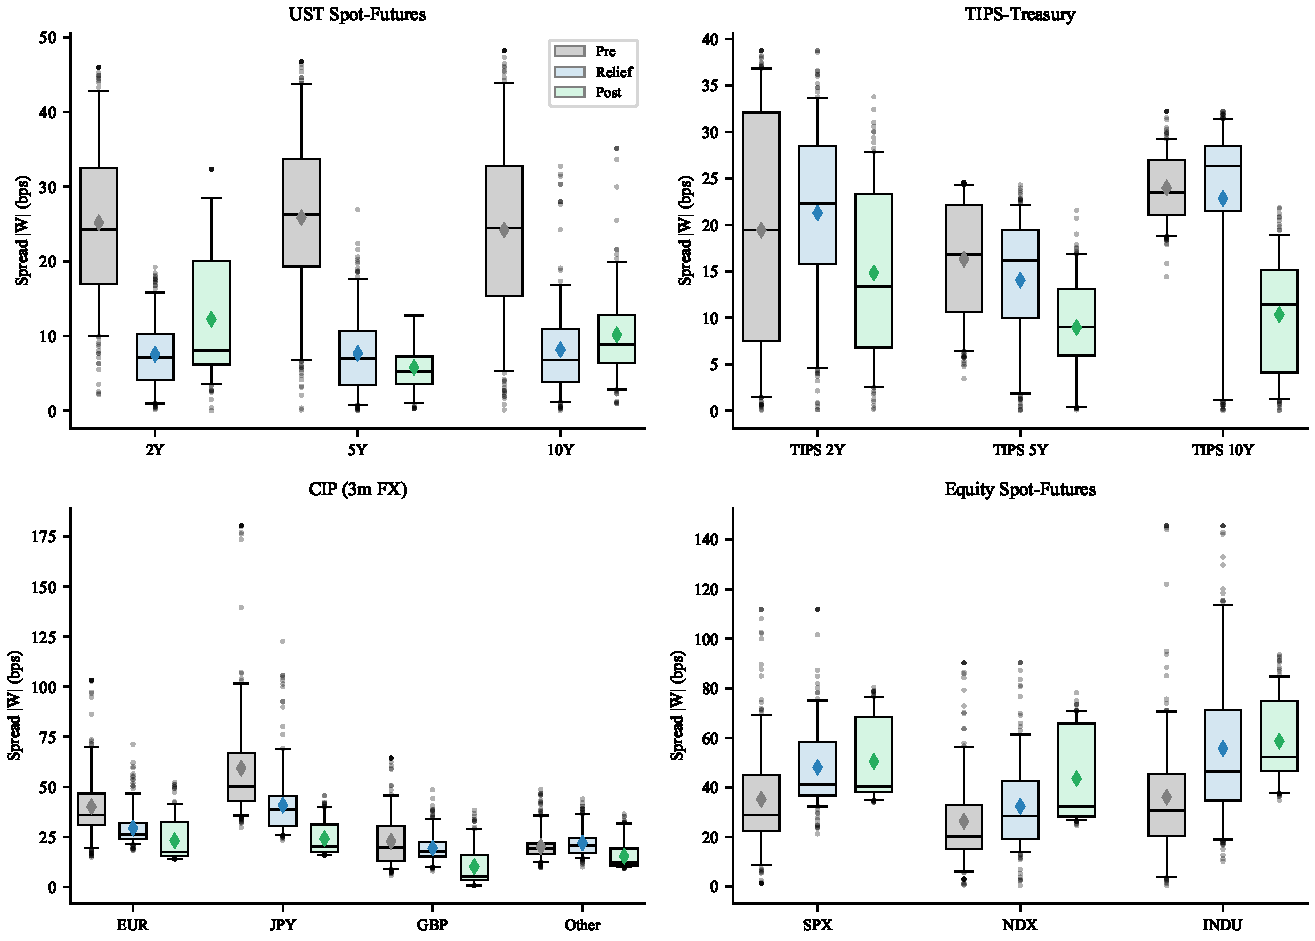
\includegraphics[width=0.95\textwidth]{../figures_output/fig6_regime_boxplots.pdf}
  \caption{Distribution of absolute arbitrage spreads $|W|$ by regime. Each
  box shows the interquartile range with median line; whiskers extend to
  1.5$\times$IQR. Treasury-based series (UST spot-futures and TIPS-Treasury)
  are shown in the left panels; non-Treasury series (CIP deviations and equity
  spot-futures) in the right panels. Regimes: Pre = January~2019 --
  March~2020; Relief = April~2020 -- March~2021; Post = April~2021 --
  December~2021 (February--March~2020 excluded from DiD regressions but
  included here for visual completeness). The sharp compression of
  Treasury-based spreads during the relief period and partial re-widening at
  expiry are visible relative to the stable non-Treasury distributions.}
  \label{fig:regime_boxplots}
\end{figure}

\begin{table}[h]
\centering
\caption{Summary Statistics for Arbitrage Spreads}
\label{tab:summary_stats}
\small
\begin{tabular}{l l r r r r r r}
\hline\hline
Strategy & Series & $N$ & Mean $\overline{W}$ & Median $W$ & Mean $|W|$ &
$Q_{0.05}(W)$ & $Q_{0.95}(W)$ \\
\hline
\multicolumn{8}{l}{\textit{Panel A: Treasury-based arbitrages (TreasuryBased $= 1$)}} \\[3pt]
TIPS--Treasury & 2y, pre   & 312 & 16.6 & 19.5 & 19.4 & $-9.7$ & 36.8 \\
               & 2y, relief & 250 & 16.8 & 22.3 & 21.4 & $-16.7$ & 33.7 \\
               & 2y, post  & 190 & 11.7 & 13.4 & 14.8 & $-11.1$ & 27.8 \\[2pt]
               & 5y, pre   & 312 & 16.3 & 16.8 & 16.3 & 6.4 & 24.3 \\
               & 5y, relief & 250 & 13.7 & 16.2 & 14.1 & $-2.1$ & 22.3 \\
               & 5y, post  & 190 & 8.7  & 9.0  &  9.0 & $-0.4$ & 16.9 \\[2pt]
               & 10y, pre  & 312 & 24.1 & 23.5 & 24.1 & 18.8 & 29.2 \\
               & 10y, relief & 250 & 22.7 & 26.3 & 22.9 & 0.1 & 31.4 \\
               & 10y, post  & 190 & 10.2 & 11.4 & 10.4 & $-0.6$ & 19.2 \\[4pt]
UST spot--fut. & 2y, pre   & 314 & $-25.4$ & $-24.3$ & 25.6 & $-43.0$ & $-9.6$ \\
               & 2y, relief & 251 & $-5.8$  & $-6.0$  &  7.6 & $-16.1$ & 9.4 \\
               & 2y, post  & 192 & 10.0  &  8.0  & 12.6 & $-3.2$ & 27.4 \\[2pt]
               & 5y, pre   & 314 & $-26.3$ & $-26.3$ & 26.4 & $-43.8$ & $-6.6$ \\
               & 5y, relief & 251 & $-6.3$  & $-6.5$  &  7.7 & $-17.8$ & 5.9 \\
               & 5y, post  & 192 & 5.5   &  5.3  &  5.8 & $-0.4$ & 12.8 \\[2pt]
               & 10y, pre  & 314 & $-20.8$ & $-23.4$ & 24.7 & $-39.1$ & 6.9 \\
               & 10y, relief & 251 & $-5.4$  & $-6.1$  &  8.2 & $-16.0$ & 7.7 \\
               & 10y, post  & 192 & 10.1  &  8.9  & 10.2 & 2.8 & 20.1 \\[4pt]
\multicolumn{8}{l}{\textit{Panel B: Non-Treasury arbitrages (TreasuryBased $= 0$, means across tenors/currencies)}} \\[3pt]
CIP 3m (8 curr.) & pre   & 326 avg.\ & --- & --- & 31.1 & --- & --- \\
                 & relief & 261 avg.\ & --- & --- & 25.9 & --- & --- \\
                 & post  & 197 avg.\ & --- & --- & 17.2 & --- & --- \\[2pt]
Equity SF (3 idx.) & pre   & 310 avg.\ & --- & --- & 32.8 & --- & --- \\
                  & relief & 248 avg.\ & --- & --- & 45.8 & --- & --- \\
                  & post  & 189 avg.\ & --- & --- & 50.9 & --- & --- \\[2pt]
\hline\hline
\end{tabular}
\begin{tablenotes}
\footnotesize
\item \textit{Notes.} Spread statistics are in basis points.
$\overline{W}$ denotes the mean signed spread; $|W|$ denotes the mean
absolute spread. Regime boundaries: pre = January 1, 2019 to March 31,
2020; relief = April 1, 2020 to March 31, 2021; post = April 1 to
December 31, 2021. CIP and equity rows report cross-series averages
within each regime. All series are winsorized at the within-series
first and 99th percentiles prior to analysis; see Table~\ref{tab:winsorize}.
\textit{Note}: the `pre' regime includes February--March 2020 (the
acute COVID crash), which are excluded from the DiD regressions
in Table~\ref{tab:pooled_jump} Panel B. Pre-period means for UST
spot-futures are therefore modestly inflated by COVID-period
observations relative to the 2019-only baseline used in the DiD.
\end{tablenotes}
\end{table}

\begin{table}[htbp]
\centering
\caption{SLR Exclusion Event Study: Pooled Jump Regressions}
\label{tab:pooled_jump}
\small
\begin{tabular}{l cccc cccc}
\hline\hline
& \multicolumn{4}{c}{Entry event (2020-04-01)$^{\dagger}$}
& \multicolumn{4}{c}{Exit event (2021-03-31)} \\
\cmidrule(lr){2-5} \cmidrule(lr){6-9}
& \multicolumn{2}{c}{$W=20$} & \multicolumn{2}{c}{$W=60$}
& \multicolumn{2}{c}{$W=20$} & \multicolumn{2}{c}{$W=60$} \\
\cmidrule(lr){2-3} \cmidrule(lr){4-5} \cmidrule(lr){6-7} \cmidrule(lr){8-9}
& \textsc{Total} & \textsc{Direct} & \textsc{Total} & \textsc{Direct}
& \textsc{Total} & \textsc{Direct} & \textsc{Total} & \textsc{Direct} \\
\hline
\multicolumn{9}{l}{\textit{Panel A: Pooled regressions}} \\[3pt]
$\mathrm{Post}$
  & $-0.84$ & $+1.45$ & $-7.08^{**}$ & $-2.76$
  & $-2.62^{***}$ & $-2.28^{***}$ & $-3.09^{***}$ & $-2.97^{***}$ \\
  & $(4.77)$ & $(7.03)$ & $(3.05)$ & $(5.54)$
  & $(0.77)$ & $(0.68)$ & $(0.83)$ & $(0.85)$ \\[3pt]
$\mathrm{Post} \times \mathrm{TreasuryBased}$
  & $-2.16$ & $-2.23$ & $-4.54$ & $-4.52$
  & $+3.91^{***}$ & $+3.90^{***}$ & $+3.84^{***}$ & $+3.84^{***}$ \\
  & $(6.13)$ & $(6.14)$ & $(3.00)$ & $(3.00)$
  & $(0.92)$ & $(0.92)$ & $(0.89)$ & $(0.88)$ \\[3pt]
$N$
  & $697$ & $697$ & $2{,}057$ & $2{,}057$
  & $697$ & $697$ & $2{,}057$ & $2{,}057$ \\
$R^{2}$
  & $0.61$ & $0.61$ & $0.55$ & $0.55$
  & $0.96$ & $0.96$ & $0.89$ & $0.89$ \\[4pt]
\hline
\multicolumn{9}{l}{\textit{Panel B: Robust DiD (2019 pre-COVID baseline, excl.\ Feb--Mar 2020)}} \\[3pt]
& \multicolumn{4}{c}{Relief period} & \multicolumn{4}{c}{Post-relief period} \\
\cmidrule(lr){2-5} \cmidrule(lr){6-9}
& \multicolumn{2}{c}{\textsc{Total}} & \multicolumn{2}{c}{\textsc{Direct}}
& \multicolumn{2}{c}{\textsc{Total}} & \multicolumn{2}{c}{\textsc{Direct}} \\
\cmidrule(lr){2-3} \cmidrule(lr){4-5} \cmidrule(lr){6-7} \cmidrule(lr){8-9}
Non-Treasury baseline
  & \multicolumn{2}{c}{$-1.34$} & \multicolumn{2}{c}{$-11.03^{***}$}
  & \multicolumn{2}{c}{$-6.92^{***}$} & \multicolumn{2}{c}{$-14.87^{***}$} \\
  & \multicolumn{2}{c}{$(1.13)$} & \multicolumn{2}{c}{$(2.97)$}
  & \multicolumn{2}{c}{$(1.01)$} & \multicolumn{2}{c}{$(2.80)$} \\[2pt]
$\times$ TreasuryBased
  & \multicolumn{2}{c}{$-10.76^{***}$} & \multicolumn{2}{c}{$-10.77^{***}$}
  & \multicolumn{2}{c}{$-9.03^{***}$} & \multicolumn{2}{c}{$-9.04^{***}$} \\
  & \multicolumn{2}{c}{$(1.15)$} & \multicolumn{2}{c}{$(1.14)$}
  & \multicolumn{2}{c}{$(1.16)$} & \multicolumn{2}{c}{$(1.16)$} \\[2pt]
$N$ & \multicolumn{4}{c}{$12{,}326$} & \multicolumn{4}{c}{$12{,}326$} \\
$R^{2}$ & \multicolumn{4}{c}{$0.516$} & \multicolumn{4}{c}{$0.516$} \\
\hline\hline
\end{tabular}
\begin{tablenotes}
\footnotesize
\item \textit{Notes.} Dependent variable is $|W_{i,t}|$, the absolute
spread in basis points. $\mathrm{Post} = 1$ for event-time $\geq 0$
within the stated $\pm W$ trading-day window. $\mathrm{TreasuryBased} = 1$
for UST spot-futures and TIPS-Treasury series. All specifications include
series fixed effects. \textsc{Total} controls: VIX, HY OAS, Baa-10y
spread. \textsc{Direct} adds SOFR, TGCR-SOFR, and rolling 7/14/30-day
Treasury issuance. HAC standard errors
(Newey-West, 5 lags) in parentheses.
${}^{***}\,p<0.01$, ${}^{**}\,p<0.05$, ${}^{*}\,p<0.10$.
${}^{\dagger}$ The entry pre-period (Jan--Mar 2020) spans the COVID-19
crash peak; entry estimates are contaminated by contemporaneous Fed
interventions. See Section~\ref{sec:entry} and Panel B (Robust DiD)
for COVID-robust estimates.
The identical $R^2 = 0.516$ across \textsc{Total} and \textsc{Direct}
in Panel~B reflects that the additional \textsc{Direct} controls (SOFR,
TGCR-SOFR, issuance) add negligible explanatory power once series fixed
effects and the broad risk controls absorb common daily variation; the
controls affect the partition of coefficients between $\hat{\mu}_1$ and
the regime dummies, not the overall fit.
The large \textsc{Direct} non-Treasury baseline during relief
($-11.03$ bps) is discussed in Section~\ref{sec:did_clean}; the
Treasury interaction $\hat{\mu}_2$ is stable across specifications
($-10.76$ vs.\ $-10.77$ bps), confirming the Treasury differential is
orthogonal to the secured funding channel.
\end{tablenotes}
\end{table}

\begin{table}[htbp]
\centering
\caption{Robustness: Total vs.\ Direct Specification Comparison}
\label{tab:robustness}
\small
\begin{tabular}{l l r r r r r r r r r r r}
\hline\hline
Event & Window & Coefficient & $N$ &
$\hat{\beta}_{\textsc{Tot}}$ & $\mathrm{SE}_{\textsc{Tot}}$ &
$t_{\textsc{Tot}}$ & Stars &
$\hat{\beta}_{\textsc{Dir}}$ & $\mathrm{SE}_{\textsc{Dir}}$ &
$t_{\textsc{Dir}}$ & $\Delta\hat{\beta}$ & $\Delta t$ \\
\hline
Entry & $W=20$ & Post & 697 & $-0.84$ & $4.77$ & $-0.18$ & --- &
  $+1.45$ & $7.03$ & $+0.21$ & $+2.29$ & $+0.38$ \\
Entry & $W=20$ & Post $\times$ Treas. & 697 & $-2.16$ & $6.13$ & $-0.35$ & --- &
  $-2.23$ & $6.14$ & $-0.36$ & $-0.06$ & $-0.01$ \\
Entry & $W=60$ & Post & 2,057 & $-7.08$ & $3.05$ & $-2.32$ & ** &
  $-2.76$ & $5.54$ & $-0.50$ & $+4.32$ & $+1.82$ \\
Entry & $W=60$ & Post $\times$ Treas. & 2,057 & $-4.54$ & $3.00$ & $-1.51$ & --- &
  $-4.52$ & $3.00$ & $-1.51$ & $+0.02$ & $+0.00$ \\[4pt]
Exit  & $W=20$ & Post & 697 & $-2.62$ & $0.77$ & $-3.40$ & *** &
  $-2.28$ & $0.68$ & $-3.33$ & $+0.34$ & $+0.06$ \\
Exit  & $W=20$ & Post $\times$ Treas. & 697 & $+3.91$ & $0.92$ & $+4.26$ & *** &
  $+3.90$ & $0.92$ & $+4.24$ & $-0.01$ & $-0.02$ \\
Exit  & $W=60$ & Post & 2,057 & $-3.09$ & $0.83$ & $-3.72$ & *** &
  $-2.97$ & $0.85$ & $-3.48$ & $+0.12$ & $+0.24$ \\
Exit  & $W=60$ & Post $\times$ Treas. & 2,057 & $+3.84$ & $0.89$ & $+4.32$ & *** &
  $+3.84$ & $0.88$ & $+4.34$ & $0.00$ & $+0.02$ \\
\hline\hline
\end{tabular}
\begin{tablenotes}
\footnotesize
\item \textit{Notes.} Each row reports both \textsc{Total} and
\textsc{Direct} estimates of the stated coefficient from
regression~(\ref{eq:did}). ``Post $\times$ Treas.'' abbreviates
$\mathrm{Post}_t \times \mathrm{TreasuryBased}_i$. Stars correspond to
the \textsc{Total} specification; \textsc{Direct} significance is
identical for all exit rows. HAC SE (Newey-West, 5 lags).
${}^{***}\,p<0.01$, ${}^{**}\,p<0.05$.
\end{tablenotes}
\end{table}

\begin{table}[htbp]
\centering
\caption{Winsorization Log: Per-Series Clipping Counts}
\label{tab:winsorize}
\small
\begin{tabular}{l l r r r r r}
\hline\hline
Series & Variable & $p_1$ bound & $p_{99}$ bound &
$n_{\text{clipped, lo}}$ & $n_{\text{clipped, hi}}$ & \% clipped \\
\hline
CIP-AUD & $|W|$ & 0.25 & 44.60 & 40 & 40 & 2.04 \\
CIP-CAD & $|W|$ & 0.24 & 45.14 & 40 & 40 & 2.04 \\
CIP-CHF & $|W|$ & 0.91 & 103.72 & 40 & 40 & 2.05 \\
CIP-EUR & $|W|$ & 1.58 & 432.41 & 40 & 40 & 2.04 \\
CIP-GBP & $|W|$ & 0.81 & 55.50 & 40 & 40 & 2.04 \\
CIP-JPY & $|W|$ & 12.67 & 110.43 & 40 & 40 & 2.05 \\
CIP-NZD & $|W|$ & 0.52 & 41.22 & 40 & 40 & 2.04 \\
CIP-SEK & $|W|$ & 1.11 & 92.02 & 40 & 40 & 2.04 \\
Eq.\ INDU & $|W|$ & 3.07 & 126.51 & 38 & 38 & 2.03 \\
Eq.\ NDX  & $|W|$ & 1.88 & 109.21 & 38 & 38 & 2.04 \\
Eq.\ SPX  & $|W|$ & 3.53 & 111.44 & 38 & 38 & 2.04 \\
TIPS 10y  & $|W|$ & 1.66 & 38.38 & 38 & 38 & 2.03 \\
TIPS 2y   & $|W|$ & 0.45 & 42.05 & 38 & 38 & 2.04 \\
TIPS 5y   & $|W|$ & 0.77 & 38.45 & 38 & 38 & 2.03 \\
UST SF 10y & $|W|$ & 0.51 & 227.33 & 50 & 50 & 2.01 \\
UST SF 2y  & $|W|$ & 0.42 & 178.09 & 50 & 50 & 2.01 \\
UST SF 5y  & $|W|$ & 0.27 & 179.19 & 50 & 50 & 2.01 \\
\hline\hline
\end{tabular}
\begin{tablenotes}
\footnotesize
\item \textit{Notes.} Each series is winsorized within-series at the first
and 99th percentiles prior to all estimation. $p_1$ and $p_{99}$ are the
clipping bounds in basis points. ``\% clipped'' reports the fraction of
observations replaced at either tail. Total clipped observations in the $|W|$ dependent variable across
the full stacked panel of 68,620 series-day pairs: approximately 1,396
(2.04 percent). The pipeline also winsorizes the signed spread $W$
separately; counting both variables gives approximately 2,792 total clips,
but the relevant figure for the estimation sample is 1,396.
\end{tablenotes}
\end{table}


\subsection{Conclusion}
\label{sec:conclusion}

This paper investigates whether regulatory leverage constraints are the operative
friction behind Treasury market arbitrage dislocations. Using the Federal
Reserve's 2020--2021 SLR exclusion as a time-dated quasi-experiment, I find
that the expiry of regulatory relief caused Treasury-based arbitrage spreads to
widen by $3.84$ basis points more than non-Treasury spreads in the subsequent
60 trading days ($t = 4.32$, $p < 0.01$), with the estimate stable to the
% SOURCE: tab:pooled_jump Panel A, Exit W=60 TOTAL, Post×TreasuryBased: coef=+3.84, SE=0.89, t=4.32 [audit_repairs/outputs/jump_estimates_pooled.csv]
one-hundredth of a basis point across control structures and robust to
cross-sectional dependence (Driscoll-Kraay $t = 5.62$). A full-period
% SOURCE: tab:dk_robustness, Exit TOTAL Post×Treas: t_DK=+5.62, SE_DK=0.683 [audit_repairs/outputs/dk_robustness.csv]
difference-in-differences recovers $-10.76$ basis points of differential
Treasury compression during the relief window relative to the 2019 pre-COVID
baseline ($t = -9.37$). Non-Treasury series---CIP deviations for eight G-10
% SOURCE: tab:did_clean Panel A, TOTAL, mu2: coef=-10.76, SE=1.15, t=-9.37 [audit_repairs/outputs/did_clean_baseline.csv]
currencies and equity spot-futures for three major indices---show no comparable
break at the SLR event dates, passing the falsification tests that are the
design's primary identification safeguard.

These results advance the work of \citet{siriwardane2025segmented}
in a specific direction. The authors document that the average pairwise correlation
among 32 arbitrage spreads is only 22 percent, inconsistent with
representative-intermediary models, and attribute this to segmented funding and
segmented balance sheets. Whereas  \citet{siriwardane2025segmented} document segmentation and attribute it
to balance-sheet constraints using cross-sectional and time-series variation
over 2010--2020, this study uses a single policy event to directly test whether
a regulatory relaxation of those constraints produces the predicted differential
response across strategy types. My results indicate that primary dealer
balance sheets are indeed marginal for Treasury spot-futures arbitrage---the
most balance-sheet-intensive of the Treasury strategies I study---and that the
regulatory effect is detectable in market prices within a 20-trading-day window.
The UST spot-futures series compressed by approximately 70 percent during the
relief period (pre-period mean $25.6$ bps to $7.8$ bps during relief), and the
cross-strategy divergence at expiry is economically meaningful relative to the
26--33 percent shadow cost of primary dealer leverage constraints estimated by
\citet{braeuning2024effect}.

The results also speak to an active policy debate. In 2025, the Federal Reserve
proposed reforms to the enhanced SLR buffer for G-SIBs that would free
substantial capital at G-SIB depository subsidiaries. The 2020--2021 episode
provides the only available quasi-experimental benchmark for the price-impact
magnitude of such a reform. My estimates suggest that a comparable structural
change in leverage capacity could compress Treasury-based arbitrage spreads by
several basis points on a sustained basis, reducing the intermediation cost
embedded in Treasury market prices.

Three extensions remain for future work. First, a bank-level mechanism test
using quarterly FR~Y-9C data would directly link the aggregate spread
compression to variation in individual banks' SLR bind, providing the
cross-sectional identification that the current design cannot. Second, the
partial reversion evidence---the point estimate from the full-period DiD
implies approximately 16 percent of the relief-period compression reversed
in the nine-month post-expiry window, though this figure is statistically
imprecise ($p = 0.11$; the 95\% CI spans essentially zero to $-3.86$ bps)---suggests that the
structural impact of the exclusion, combined with concurrent Fed balance sheet
expansion and the launch of the Standing Repo Facility, may have durably
improved Treasury market intermediation in ways that outlasted the formal
regulation. Third, a local projections specification would allow the impulse
response of each spread to be estimated flexibly over post-event horizons,
which would be informative about the speed of arbitrage capital reallocation
following the regulatory change.

% ── Bibliography ──────────────────────────────────────────────────────────
% natbib is loaded above (\usepackage{natbib}).
% Use \citet{key} for inline "Author (Year)" and \citep{key} for "(Author, Year)".
%
% Style options (uncomment one):
%   plainnat  — author-year, alphabetical, always available with natbib
%   abbrvnat  — author-year, abbreviated first names
%   jf        — Journal of Finance style (requires jf.bst to be installed)
%
\bibliographystyle{plainnat}
%
% All BibTeX entries are in presentations/references.bib
% Cite keys used in this section:
%   siriwardane2025segmented, du2018deviations, fleckenstein2014tips,
%   he2017intermediary, callaway2021difference, driscoll1998consistent,
%   liang2020enhancing, favara2024leverage, braeuning2024effect, cochran2023dealers
% NOTE: favara2024leverage has VERIFY flag — confirm journal publication status.

\bibliography{nsf_references}
\end{document}